\documentclass[]{styles/svproc}  % Comment this line out

%\IEEEoverridecommandlockouts                              % This command is only
                                                          % needed if you want to
                                                          % use the \thanks command
%\overrideIEEEmargins

\usepackage{amsmath}    % need for subequations
\usepackage{amssymb}
\usepackage{graphicx}   % need for figures
\usepackage{color}      % use if color is used in text
\usepackage{subcaption}
\captionsetup{compatibility=false}
\usepackage{algorithm}
\usepackage{algpseudocode}
\usepackage{url}
\usepackage{bm}
\usepackage[outdir=./figures/]{epstopdf}
\def\UrlFont{\rmfamily}
\usepackage{tikz}
\usetikzlibrary{through,calc, quotes,angles}
\usepackage{mathtools}


% bounce transition graph
% visibility event graph
% bounce visibility diagram/graph

% synthesis of paths with high-level dynamical properties from simple
% compliant environmental interactions

% skeptical questions:

% - what if the robot starts very near to a boundary of equivalence classes?
% - why not just use wall-following?

% Using Visibility Equivalence Classes for High-Level Dynamical Path Synthesis

% Minimal (Complexity | Attention) Path Synthesis with Dynamical Specifications

%\title{Path Synthesis from Dynamical Specifications \\ for Blind Mobile Robots in Polygons}
\addtolength{\belowcaptionskip}{-1em}
%
%
%
%%%% list of authors for the TOC (use if author list has to be modified)
%\tocauthor{Ivar Ekeland, Roger Temam, Jeffrey Dean, David Grove,
%Craig Chambers, Kim B. Bruce, and Elisa Bertino}
%

\begin{document}
\mainmatter              % start of a contribution


% A Toolbox for
\title{A Visibility-Based Approach to Computing Nondeterministic Bouncing
Strategies}

\titlerunning{Nondeterministic Bouncing Strategies}  % abbreviated title (for running head)
%                                     also used for the TOC unless
%                                     \toctitle is used
\author{Alexandra Q. Nilles\inst{1} \and Yingying Ren\inst{1} \and Israel
Becerra\inst{1} \and Steven M. LaValle\inst{2,1}% <-this % stops a space
}
\institute{Department of Computer Science \\
University of Illinois at Urbana-Champaign, Urbana, IL 61801 USA\\
\email{\{nilles2, yren17, israelb4, lavalle\}@illinois.edu}\\ 
\and
Faculty of Information Technology and Electrical Engineering\\
University of Oulu, Oulu, Finland
}
\authorrunning{A. Nilles, Y. Ren, I. Becerra, S. M. LaValle} % abbreviated author list (for running head)
%\email{I.Ekeland@princeton.edu},\\ WWW home page:
%\texttt{http://users/\homedir iekeland/web/welcome.html}
%\and
%Universit\'{e} de Paris-Sud,
%Laboratoire d'Analyse Num\'{e}rique, B\^{a}timent 425,\\
%F-91405 Orsay Cedex, France}


\maketitle

%%%%%%%%%%%%%%%%%%%%%%%%%%%%%%%%%%%%%%%%%%%%%%%%%%%%%%%%%%%%%%%%%%%%%%%%%%%%%%%%
\begin{abstract}
Inspired by motion patterns of some commercially available mobile robots, we
investigate the power of robots that move forward in straight lines until
colliding with an environment boundary, at which point they can rotate in place
and move forward again; we visualize this as the robot ``bouncing'' off
boundaries. Different boundary interaction rules can be defined for such robots,
such as one that orients the robot relative to its heading prior to collision,
or relative to the normal of the boundary. We introduce a new data structure,
the {\em bounce visibility graph}, which is generated from a polygonal
environment definition. The bounce visibility graph can be queried to determine
the feasibility of path-based tasks such as navigation and patrolling, assuming
we have unavoidable nondeterminism in our actuation. If the task is feasible, 
then this approach synthesizes a strategy (a sequence of nondeterministic rotations). We also show how to compute
stable cyclic trajectories and use these to limit uncertainty in the robot's
position.
\footnote{Code and documentation available at
\url{https://github.com/alexandroid000/bounce_viz}}
\end{abstract}


\section{Introduction}

Mobile robots have rolled smoothly into our everyday lives, and can now be
spotted vacuuming our floors, cleaning our pools, mowing our grass, and moving
goods in our warehouses. These tasks require that the robot's path achieve certain properties; for example, a 
vacuuming robot should cover the whole space while not visiting 
any particular area more frequently than others. A robot that is monitoring
humidity or temperature in a warehouse should repeat its path consistently so data 
can be compared over time. In many such examples, the strategies for controlling 
the robot's path may be decoupled from the specific application, so we envision building a
library of useful high-level path controllers based on desired dynamical system
properties.

Current algorithmic approaches to these tasks take two flavors: 1) maximizing
the information available to the robot though high-fidelity sensors and
map-generating algorithms such as SLAM, or 2) minimizing the information needed
by the robot, such as the largely random navigation strategies of the early
robot vacuums. The first approach is powerful and well-suited to dynamic
environments, but also resource-intensive in terms of energy, computation, and
storage space. The second approach is more resource efficient, but does not
immediately provide general-purpose strategies for navigation and loop-closure.
We propose a combined approach: first, global geometry of environment boundaries
is provided to the system, either \emph{a priori} or calculated online by an
algorithm such as SLAM. The global geometry is then processed to produce a
strategy providing strong formal guarantees and which can be executed with
minimal processing power and only low bandwidth local sensors, such as bump and
proximity sensors, instead of high bandwidth sensors such as cameras.

In this paper, we consider simple robots with ``bouncing" behaviors: robots that
travel in straight lines in the plane, until encountering an environment
boundary, at which point they rotate in place and set off again. The exact
action taken at a boundary will be determined by what we call {\em bounce rules}.
A growing line of work is considering the computational power of individual
bounce rules and their applications to robotic tasks in biological, microscale, 
and dynamical contexts. The environment interactions may be mechanical,
with the robot actually making contact with a surface, or may be simulated with
virtual boundaries such as the perimeter wire systems used by lawn mowing robots
\cite{sahin2007household}. Physical implementations of the bouncing maneuver have
been validated experimentally, for example in \cite{alam2018space} and \cite{LewOKa13}. 
Often these lines of work consider only a small
part of the strategy space, such as an iterated fixed bounce rule. In this work, 
we present a tractable approach to reasoning over {\em all possible} bounce strategies,
generalizing previous tools for analyzing a few given bounce rules.

This paper presents three ideas for simplifying the characterization and
generation of paths of such mobile robots. One crucial
aspect of our approach is that we assume that the robot has some intrinsic
nondeterminism, so we generate nondeterministic strategies such that if the
robot executes any action in a family at each stage, the strategy will succeed.
We can then analyze the size of the families of bounce rules at each stage to
determine the minimum required accuracy of a successful robot design.
Our second contribution is that by using the geometric
structure of a polygonal environment, we can create a combinatorial
representation of the environment that lets us reason over a finite number of
families of paths, instead of the infinite collection of all possible paths.
Finally, we provide results on when transitions in this robotic system are 
\emph{contracting}: two potential robot states under the transition move closer together. 
This property can be used to control uncertainty through actuation, and we
provide the first steps toward synthesizing strategies which leverage this
property.

\begin{figure}
\centering
\begin{subfigure}{0.5\textwidth}
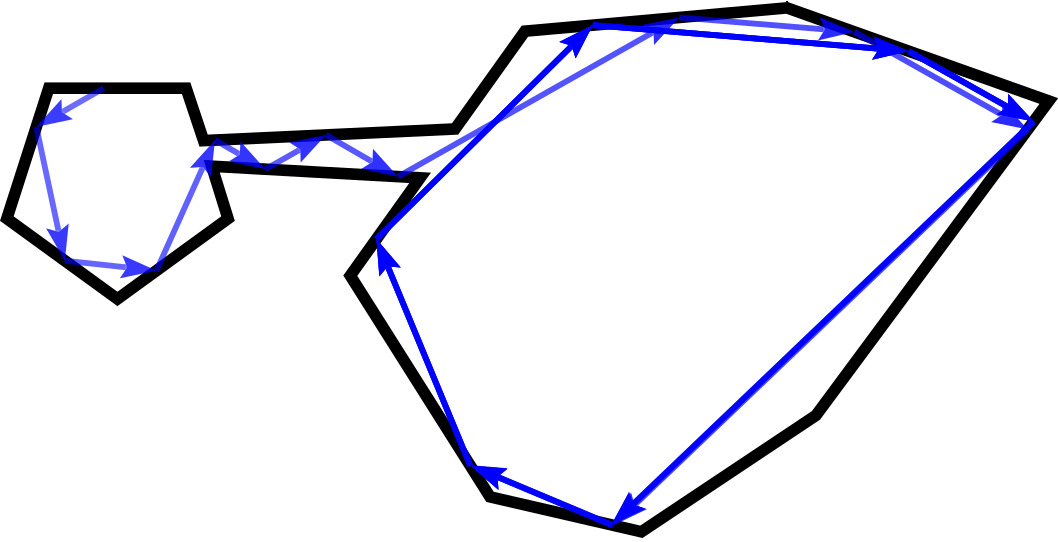
\includegraphics[width=\linewidth]{figures/twoc_a}
\end{subfigure}%
\begin{subfigure}{0.5\textwidth}
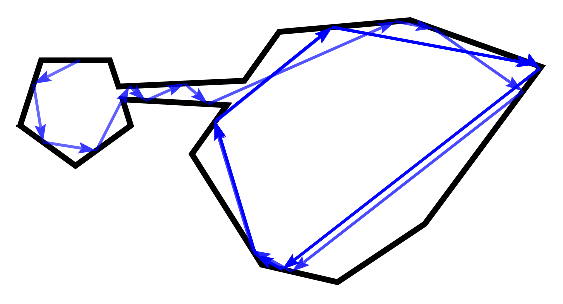
\includegraphics[width=\linewidth]{figures/twoc_b}
\end{subfigure}
\caption{Two paths produced by different sequences of bounces, which visit
different points of $\partial P$, yet have the same sequence of edge collisions 
and high-level dynamical behavior (escape the room on the left, travel through hallway, then
patrol the room on the right in a periodic orbit).
}

\label{fig:twopaths}
\end{figure}

\section{Related Work}

We incorporate techniques from computational geometry, specifically visibility
\cite{ghosh2007visibility}. Visibility has been considered extensively in
robotics, but usually with the goal of avoiding obstacles
\cite{lozano1979algorithm,SimLauNis00}. To plan over collisions, we use the edge
visibility graph, analyzed in \cite{rourke_viz}, and shown to be strictly more
powerful than the vertex visibility graph. Our work is also related to problems
that consider what parts of a polygon will be illuminated by a light source
after multiple reflections (as if the edges of the polygon are mirrors)
\cite{Aronov1996}, or with diffuse reflections \cite{prasad1998visibility},
which are related to our nondeterministic bounces.

The dynamical system defined by our robot model is related to
\emph{dynamical billiards} \cite{billiards}. Along with specular reflection,
modified dynamical systems have also attracted recent interest
\cite{DelMagno2014,pinball,billiards}. One very similar work was inspired by the
dynamics of microorganisms; in \cite{microorganism2017}, the authors show that
\textit{Chlamydomonas reinhardtii} ``bounce'' off boundaries at a specific
angle determined by their body morphology. They characterize periodic and
chaotic trajectories of such agents in regular polygons, planar curves, and
other environments.

Our motion model is a
form of \emph{compliant motion}, in which task constraints are used to guide task
completion, even when the exact system state is not known. Our use of
contraction mappings and nondeterministic reasoning is
related to the idea of funnelling: using
the attraction regions of a dynamical system to guide states into a goal region.
These ideas have been developed in the context of manipulation and fine motion control by Whitney
\cite{Whi77}, Mason \cite{Mas85}, Erdmann
\cite{Erd86}, Goldberg \cite{Gol93}, Lozano-P{\'e}rez, Mason, and Taylor
\cite{LozMasTay84}, Lynch and Mason \cite{LynMas95}, and Burridge, Rizzi, and Koditschek
\cite{BurRizKod99}, among many others.

Our intentional use of collisions with
environment boundaries is enabled by the advent of more robust, lightweight mobile
robots. Collisions as information sources have also been
recently explored for multi-robot systems \cite{mayya2018localization}. Our
specific motion model has been used in works such as \cite{OkaLav06} to
determine minimal information processing requirements for mobile robot tasks.
The first-class study of the dynamical properties of bouncing was proposed in
\cite{ErLav13} and continued in \cite{NilBecLav17}. Here we extend and improve
these analysis tools, and incorporate visibility properties to
discretize the strategy space.

In \cite{alam2017minimalist} and \cite{alam2018space}, the authors describe
navigation, coverage, and localization algorithms for a robot that rotates a fixed amount 
relative to the robot's prior heading. The
algorithm is complete and correct up to discretization, though periodic
trajectories may exist which require bounce angles not allowed by the
discretization. By using a discretization induced by the environment geometry,
we are able to find all possible limit cycles, and the controllers necessary to
achieve them.
Another very closely related work is \cite{LewOKa13}, which considered
navigation for a robot that moves in a straight line until encountering an
environment boundary, then rotates in place with uncertainty, given as input to the
algorithm. Instead of taking this parameter as input, our approach
considers all possible amounts of uncertainty, and returns bounds on the required
accuracy of movement.

We are working toward a generalization and hierarchy of robot models, in a
similar spirit to \cite{brunner2008simple}. Their {\em simple
combinatorial robot} is able to detect all visible vertices and any edges
between them, and move straight toward vertices. By augmenting this basic robot model
with sensors they construct a hierarchy of these robot models. Our questions are related but
different: if the robot is given a compact, purely combinatorial environment representation, 
what tasks can it accomplish with minimal sensing?

\section{Model and Definitions}

We consider the movement of a point robots in simple 
polygonal environments. All index arithmetic for polygons with $n$ vertices is mod $n$ 
throughout this paper. We do not require polygons in general position. We do
not consider trajectories that intersect polygon vertices.. We define our robot to move forward in a straight line, until
encountering an environment boundary (such as when a bump or range sensor is
triggered). Once at a boundary, the robot is able to rotate in place.

More formally, the model is:
\begin{itemize}
\item The \emph{configuration space} $X = \partial P \times S^1$. $P$ is a simple polygon,
potentially with hole set $O$, with boundary $\partial P$, the external boundary
unioned with the boundaries of the obstacles. $S^1$ is the robot's orientation in the plane. For the most part, one can ignore configurations in the interior
of the polygon and only consider transitions between points and intervals on the
boundary. Let $s$ refer to a point in $\partial P$ without an associated robot orientation.
\item The \emph{action space} $U = [0,\pi]$, in which $u \in U$ is executed when
the robot is in contact with an environment boundary; $u$ is measured counterclockwise
relative to the boundary. The action of departing the boundary while oriented at the boundary
normal corresponds to $u = \pi/2$.
\item The \emph{state transition function} $f: X \times U \to X$, which
describes how the state of the robot changes according to which action is
chosen. We will often lift this function to act nondeterministically over sets
of states and actions, propagating each state forward with each possible action,
and unioning the resulting set of states. 
\item We model time as proceeding in stages; at each stage $k$, the robot
is in contact with the environment boundary, executes an action $u_k$, and then
moves forward until the next contact with the boundary at stage $k+1$.
\end{itemize}

\begin{figure}
    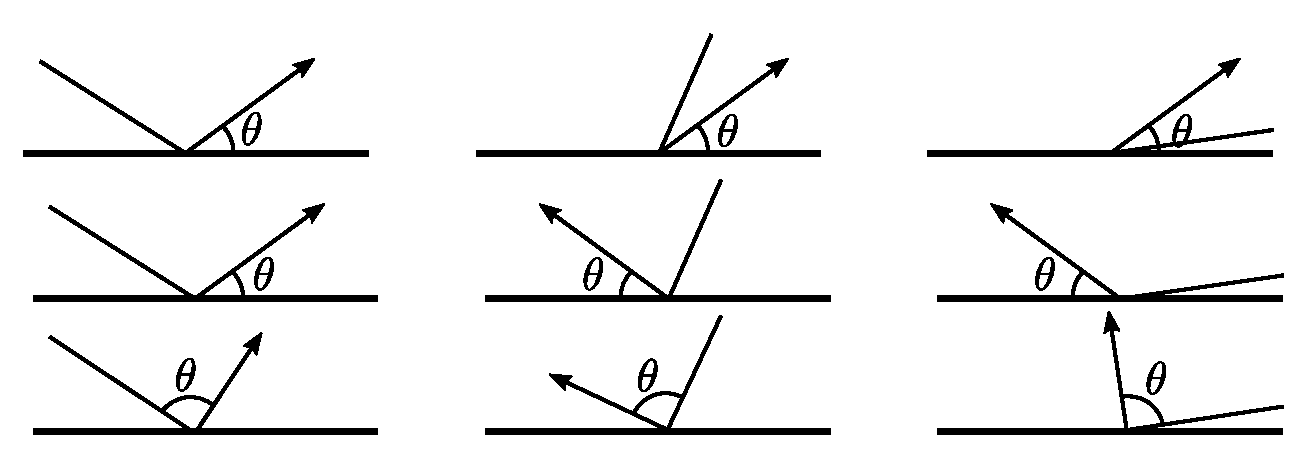
\includegraphics[width=0.8\linewidth]{figures/bounce_examples.pdf}
    \centering
    \caption[test]{\label{fig:bex}Examples of different ``bounce rules'' that can be implemented on
mobile robots. In the first row, $b(\alpha, \theta) = \theta$, which we refer to
as a \textbf{fixed} bounce rule. In the second row, we have a \textbf{monotonic
fixed} bounce rule, in which
$b(\alpha, \theta) = \theta$ or $\pi-\theta$, depending on what is necessary to
preserve monotonicity of travel direction along the $x$ axis. In the third
row, we have a \textbf{relative} bounce rule, $b(\alpha, \theta) = \alpha - \theta$, rotating $\alpha$ through $\theta$ in the clockwise
direction. If this rotation causes the 
heading of the robot to still be facing into the boundary, the robot 
performs the rotation again until its heading points into the free space.
}
\end{figure}

\begin{definition}
Let $\alpha \in (0,\pi)$ be the robot's incoming heading relative to the
environment boundary at the point of contact. Let $\theta \in (0,\pi)$ be a control parameter. A 
\textbf{bounce rule} $b$ maps $\alpha$ and $\theta$ to an action
$u$, and determines how the robot will reorient itself when it collides with a
boundary. Bounce rules are defined in the
frame in which the environment normal is aligned with the positive $y$ axis and the
robot's point of contact with the boundary is the origin.
\end{definition}
\begin{definition}
A \textbf{nondeterministic bounce rule} is a bounce rule lifted to return a set of actions. 
We will restrict nondeterministic bounce rules to
return a convex set of actions (a single interval in $(0, \pi)$).
\end{definition}

For example, a specular bounce (laser beams, billiard balls) has bounce rule 
$b(\alpha, \theta) = \pi - \alpha$. See Figure \ref{fig:bex} for more
examples of bounce rules. 

\begin{definition}
A \textbf{bounce strategy} is a sequence of nondeterministic bounce rules.
\end{definition}

Of course, robots rarely move perfectly, so our analysis will assume the
robot has some nondeterminsim in its motion execution.
Instead of modelling explicit
distributions, our definition of bounce strategy will provide design constraints
for robots capable of executing the strategies. For example, if a robot told to
perform action $u$ acutally executes
an action in the range $u \pm \epsilon$, the largest allowable $\epsilon$ will be half the
width of the smallest interval in a strategy.


\section{Visibility-Based Boundary Partitioning} \label{sec:partition}

Given a polygonal environment (such as the floor plan of a warehouse or office
space), we would like to synthesize bounce strategies that allow a robot to
perform a given task (such as navigation or patrolling).
To do so, we first discretize the continuous space of all possible
transitions between points on $\partial P$. We find a visibility-based partition
that encodes the idea of some points on $\partial P$ having different
available transitions.

\begin{definition}
The \textbf{visibility polygon} of a point $s$ in a polygon $P$ is the polygon
formed by all the points in $P$ that can be connected to $s$ with a line
segment that lies entirely within $P$.
\end{definition}
%%S Are there any open/closed set issues with this?  Ambiguous?

Imagine a robot sliding along the boundary of a polygon, calculating 
the visibility polygon as it moves. In a convex polygon, nothing exciting 
happens. In a nonconvex polygon, the reflex vertices (vertices with an
internal angle greater than $\pi$) cause interesting
behavior.
As the robot slides, its visibility polygon mostly changes continuously. Edges
shrink or grow, but the combinatorial structure of the polygon remains the same,
until it aligns with a reflex vertex $r$ and another vertex $v$ (visible
from $r$). At this point, either 
$v$ will become visible to the robot, adding an edge to the visibility 
polygon, or $v$ will disappear behind $r$, removing an edge from the visibility polygon.

To compute all such points at which the visibility polygon changes structure, we
 compute the \textbf{partial local sequence}, defined in \cite{rourke_viz}.
Each point in the partial local sequence marks the point
at which a visible vertex appears or disappears behind a reflex vertex.
The sequence is constructed by shooting a ray through each reflex vertex $r$ from every
visible vertex and keeping the resulting sequence of intersections with
$\partial P$. See Figure \ref{fig:alg1} for an
example of the vertices in the partial local sequence of $v_0$. 

Once all the partial local sequences have been inserted into the original
polygon, the resulting points along the boundary define segments for which 
any two points in the segment can see the same edge set of the
original polygon (though they may see different portions of those edges).
Thus, the set of possible transitions from a segment becomes easier to
characterize discretely. See Algorithm \ref{algo:insert} for a pseudocode
description of this partitioning process. Algorithm
\ref{algo:insert} applies to polygons with or without holes; holes simply
require a bit more bookkeeping to correctly find visible vertices and shoot
rays. Let $P'$ be the polygon $P$ after application of Algorithm
\ref{algo:insert}.

\begin{algorithm}
\caption{\textsc{PartitionPoly}(P)}
\label{algo:insert}
\hspace*{\algorithmicindent} \textbf{Input:} A polygon $P$ as a list of
vertices in counterclockwise order.\\
\hspace*{\algorithmicindent} \textbf{Output:} $P'$: $P$ with
all partial local sequence points added as new vertices.
\begin{algorithmic}[1]
\State $v_{new} \gets \{\}$
\State $reflex\_verts \gets$ \Call{GetReflexVerts}{$P$}
\For{$v_r$ in $reflex\_verts$}
    \For{$v_{vis}$ in \Call{VisibleVerts}{$P, v_r$}} 
        \State $v_{new} \gets$ $v_{new} \cup$ \Call{ShootRay}{$v_{vis}, v_r$}
    \EndFor
\EndFor
\State $P' \gets$ \Call{InsertVerts}{$v_{new}, P$}
\State \textbf{return} $P'$
\end{algorithmic}
\end{algorithm}

The $\textsc{ShootRay}$ function takes two visible vertices $v_{1}$ and $v_{2}$
and compute the first intersection of $\partial P$ and ray $v_{1}v_{2}$. This
operation will take $O(\log n)$ time after preprocessing the polygon $P$ in
$O(n)$ \cite{Szirmay-Kalos:1998:WVA:297217.297219}. The $\textsc{VisibleVerts}$
function computes all visible vertices in the polygon given an input query
vertex, and takes $O(n)$ \cite{ElGindy1981ALA}. So the total runtime of
Algorithm 1 is $O(n^2\log n)$.

\begin{definition}
The \textbf{edge visibility graph} of a polygon $P$ has a node for each edge of
$P$, and has an arc between two nodes $(e_i, e_j)$ if and only if there is a
point $s_i$ in the open edge $e_i$ and a point $s_j$ on the open edge $e_j$ such
that $s_i$ and $s_j$ can be connected with a line segment which is entirely
within the interior of $P$.
\end{definition}

%\begin{definition}
%Let $\thicksim$ be an equivalence relation such that for $s_1, s_2 \in \partial
%P$, $s_1 \thicksim s_2$ if and only if the visibility polygons of $s_1$ and $s_2$ have
%the same .
%\end{definition}
%
%This relation satisfies the necessary
%properties {\color{red} todo but easy},
%
%\begin{itemize}
%\item reflexivity
%\item symmetry
%\item transitivity
%\end{itemize}
%
%The partition of $\partial P$ created by Algorithm \ref{algo:insert} are the
%equivalence classes induced by $\thicksim$ {\color{red} todo but easy}.

\setlength{\intextsep}{5pt}
\begin{figure}[h]
\centering
\begin{subfigure}{0.5\textwidth}
    \centering
    \resizebox {\columnwidth} {!} {
    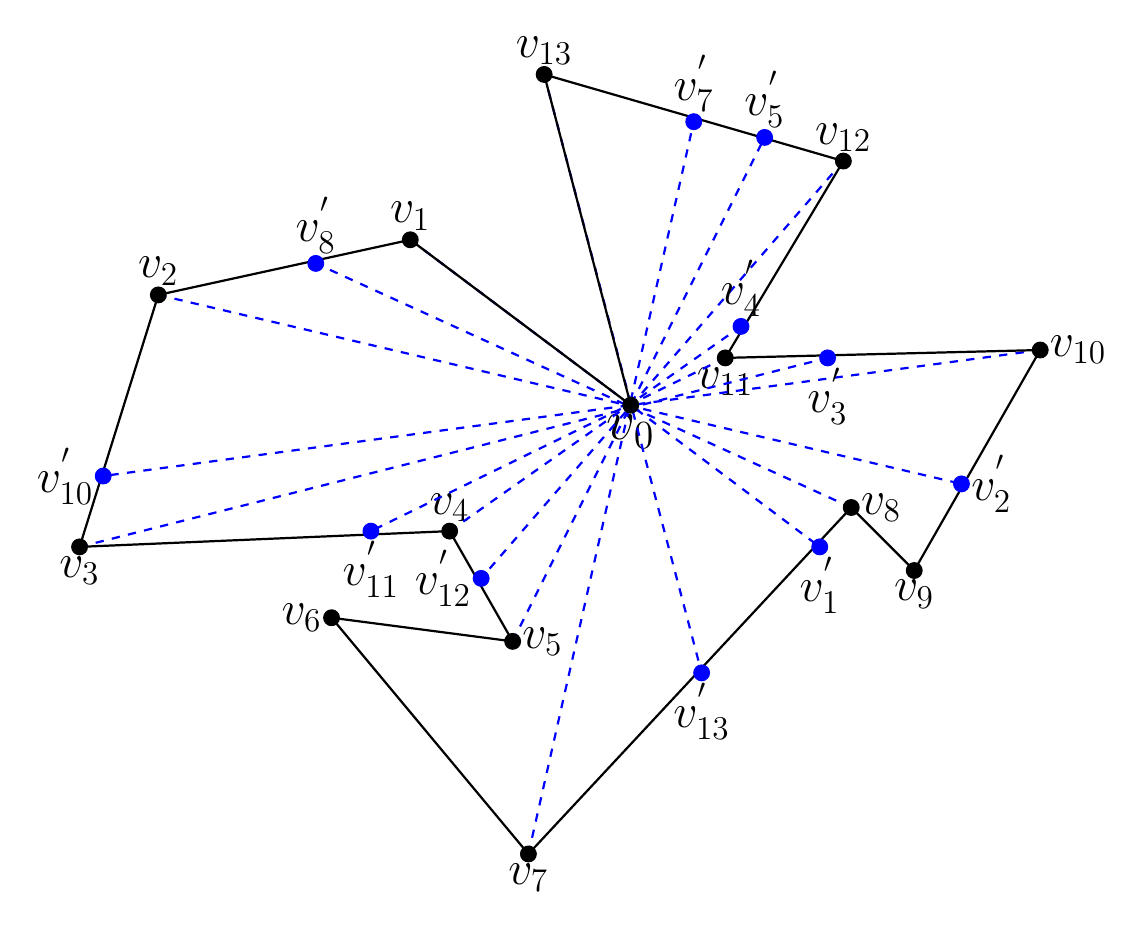
\begin{tikzpicture}
      \coordinate (A) at (-4.7, 2.4);
      \coordinate (B) at (-5.7, -0.8);
      \coordinate (C) at (-1,-0.6);
      \coordinate (D) at (-0.2,-2);
      \coordinate (E) at (-2.5, -1.7);
      \coordinate (F) at (0, -4.7);
      \coordinate (G) at (4.1, -0.3);
      \coordinate (H) at (4.9, -1.1);
      \coordinate (I) at (6.5, 1.7);
      \coordinate (J) at (2.5, 1.6);
      \coordinate (K) at (4, 4.1);
      \coordinate (L) at (0.2, 5.2);
      \coordinate (M) at (1.3, 1);
      \coordinate (N) at (-1.5, 3.1);
      \node at (A) [above] {\LARGE $v_2$};
      \node at (B) [below] {\LARGE $v_3$};
      \node at (C) [above] {\LARGE $v_4$};
      \node at (D) [right] {\LARGE $v_5$};
      \node at (E) [left] {\LARGE $v_6$};
      \node at (F) [below] {\LARGE $v_7$};
      \node at (G) [right] {\LARGE $v_8$};
      \node at (H) [below] {\LARGE $v_9$};
      \node at (I) [right] {\LARGE $v_{10}$};
      \node at (J) [below] {\LARGE $v_{11}$};
      \node at (K) [above] {\LARGE $v_{12}$};
      \node at (L) [above] {\LARGE $v_{13}$};
      \node at (M) [below] {\huge $v_0$};
      \node at (N) [above] {\LARGE $v_1$};

      \coordinate (A') at (5.5, 0);
      \coordinate (B') at (3.8, 1.6);
      \coordinate (C') at (2.7, 2);
      \coordinate (D') at (3, 4.4);
      \coordinate (F') at (2.1, 4.6);
      \coordinate (G') at (-2.7, 2.8);
      \coordinate (I') at (-5.4, 0.1);
      \coordinate (J') at (-2, -0.6);
      \coordinate (K') at (-0.6, -1.2);
      \coordinate (L') at (2.2, -2.4);
      \coordinate (N') at (3.7, -0.8);

      \draw [thick, dashed, blue] (A) -- (A');
      \draw [thick, dashed, blue] (B) -- (B');
      \draw [thick, dashed, blue] (C) -- (C');
      \draw [thick, dashed, blue] (D) -- (D');
      \draw [thick, dashed, blue] (F) -- (F');
      \draw [thick, dashed, blue] (G) -- (G');
      \draw [thick, dashed, blue] (I) -- (I');
      \draw [thick, dashed, blue] (J) -- (J');
      \draw [thick, dashed, blue] (K) -- (K');
      \draw [thick, dashed, blue] (L) -- (L');
      \draw [thick, dashed, blue] (N) -- (N');

      \draw [fill] (A) circle [radius = 0.1];
      \draw [fill] (B) circle [radius = 0.1];
      \draw [fill] (C) circle [radius = 0.1];
      \draw [fill] (D) circle [radius = 0.1];
      \draw [fill] (E) circle [radius = 0.1];
      \draw [fill] (F) circle [radius = 0.1];
      \draw [fill] (G) circle [radius = 0.1];
      \draw [fill] (H) circle [radius = 0.1];
      \draw [fill] (I) circle [radius = 0.1];
      \draw [fill] (J) circle [radius = 0.1];
      \draw [fill] (K) circle [radius = 0.1];
      \draw [fill] (L) circle [radius = 0.1];
      \draw [fill] (M) circle [radius = 0.1];
      \draw [fill] (N) circle [radius = 0.1];

      \draw [thick] (A) -- (B);
      \draw [thick] (B) -- (C);
      \draw [thick] (C) -- (D);
      \draw [thick] (D) -- (E);
      \draw [thick] (E) -- (F);
      \draw [thick] (F) -- (G);
      \draw [thick] (G) -- (H);
      \draw [thick] (H) -- (I);
      \draw [thick] (I) -- (J);
      \draw [thick] (J) -- (K);
      \draw [thick] (K) -- (L);
      \draw [thick] (L) -- (M);
      \draw [thick] (M) -- (N);
      \draw [thick] (N) -- (A);

      \node at (A') [right] {\LARGE $v_{2}^{'}$};
      \node at (B') [below] {\LARGE $v_{3}^{'}$};
      \node at (C') [above] {\LARGE $v_{4}^{'}$};
      \node at (D') [above] {\LARGE $v_{5}^{'}$};
      \node at (F') [above] {\LARGE $v_{7}^{'}$};
      \node at (G') [above] {\LARGE $v_{8}^{'}$};
      \node at (I') [left] {\LARGE $v_{10}^{'}$};
      \node at (J') [below] {\LARGE $v_{11}^{'}$};
      \node at (K') [left] {\LARGE $v_{12}^{'}$};
      \node at (L') [below] {\LARGE $v_{13}^{'}$};
      \node at (N') [below] {\LARGE $v_{1}^{'}$};
      \draw [fill, blue] (A') circle [radius = 0.1];
      \draw [fill, blue] (B') circle [radius = 0.1];
      \draw [fill, blue] (C') circle [radius = 0.1];
      \draw [fill, blue] (D') circle [radius = 0.1];
      \draw [fill, blue] (F') circle [radius = 0.1];
      \draw [fill, blue] (G') circle [radius = 0.1];
      \draw [fill, blue] (I') circle [radius = 0.1];
      \draw [fill, blue] (J') circle [radius = 0.1];
      \draw [fill, blue] (K') circle [radius = 0.1];
      \draw [fill, blue] (L') circle [radius = 0.1];
      \draw [fill, blue] (N') circle [radius = 0.1];
      % \draw [thick](A) -- (B) node [midway, below, font = \large] {$e_i$};
      % \draw [thick](B) -- (C);
      % \draw[thick, dotted] (A) -- (C);
    \end{tikzpicture}
    }
\end{subfigure}%
\begin{subfigure}{0.4\textwidth}
    \centering
    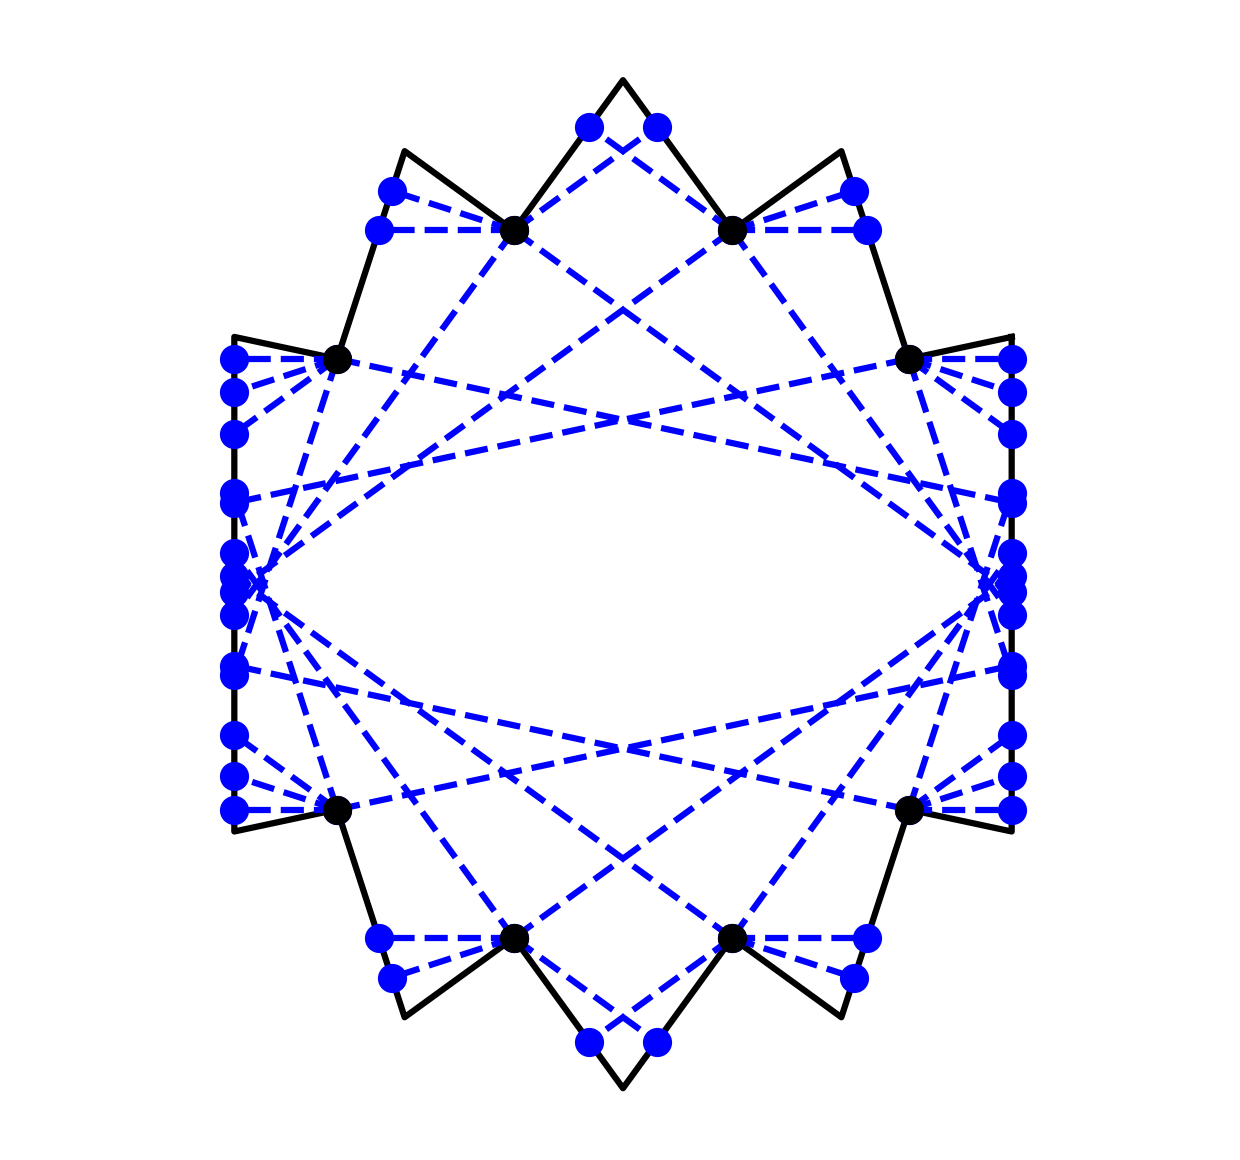
\includegraphics[width=\linewidth]{figures/chestnut_5.png}
\end{subfigure}
\centering
\caption{On the left, the partial local sequence for $v_0$. On the right, an example polygon for which the bounce visibility graph has
$O(n^4)$ edges.\label{fig:alg1}}
\end{figure}

\begin{definition}
Let the \textbf{bounce visibility graph} be the directed edge visibility graph of
$P'$.
\end{definition}

Although visibility is a symmetric property, we use directed edges in the
bounce visibility graph so that 
we can model the 
geometric constraints on the visibility from one edge to another, which are
not symmetric and govern what actions allow the robot to accomplish that
transition. See Section \ref{sec:safe} for further exploration of this idea.

We now define the \textbf{bounce visibility diagram}, a
representation of the vertex-edge visibility structure of a partitioned polygon $P'$.
%This representation
%was inspired by link diagrams \cite{efrat2000sweeping,tan_sweep}.
If $|\partial P'|$ is the perimeter length of $\partial P'$, let the $x$ axis of the
bounce visibility diagram be the interval $[0, |\partial P'|)$, in which the
endpoints of the interval are identified. Let the $y$ axis of the diagram be a
parameter $\theta$, which is an angle between $0$ and $\pi$.
For a point $s \in \partial P'$, we can compute all the visible vertices and
the angle at which they are visible. The graph of all angles at which vertices
are visible from points in $\partial P'$ is the bounce visibility diagram.

\begin{figure}
\centering
\begin{subfigure}{0.5\textwidth}
\centering
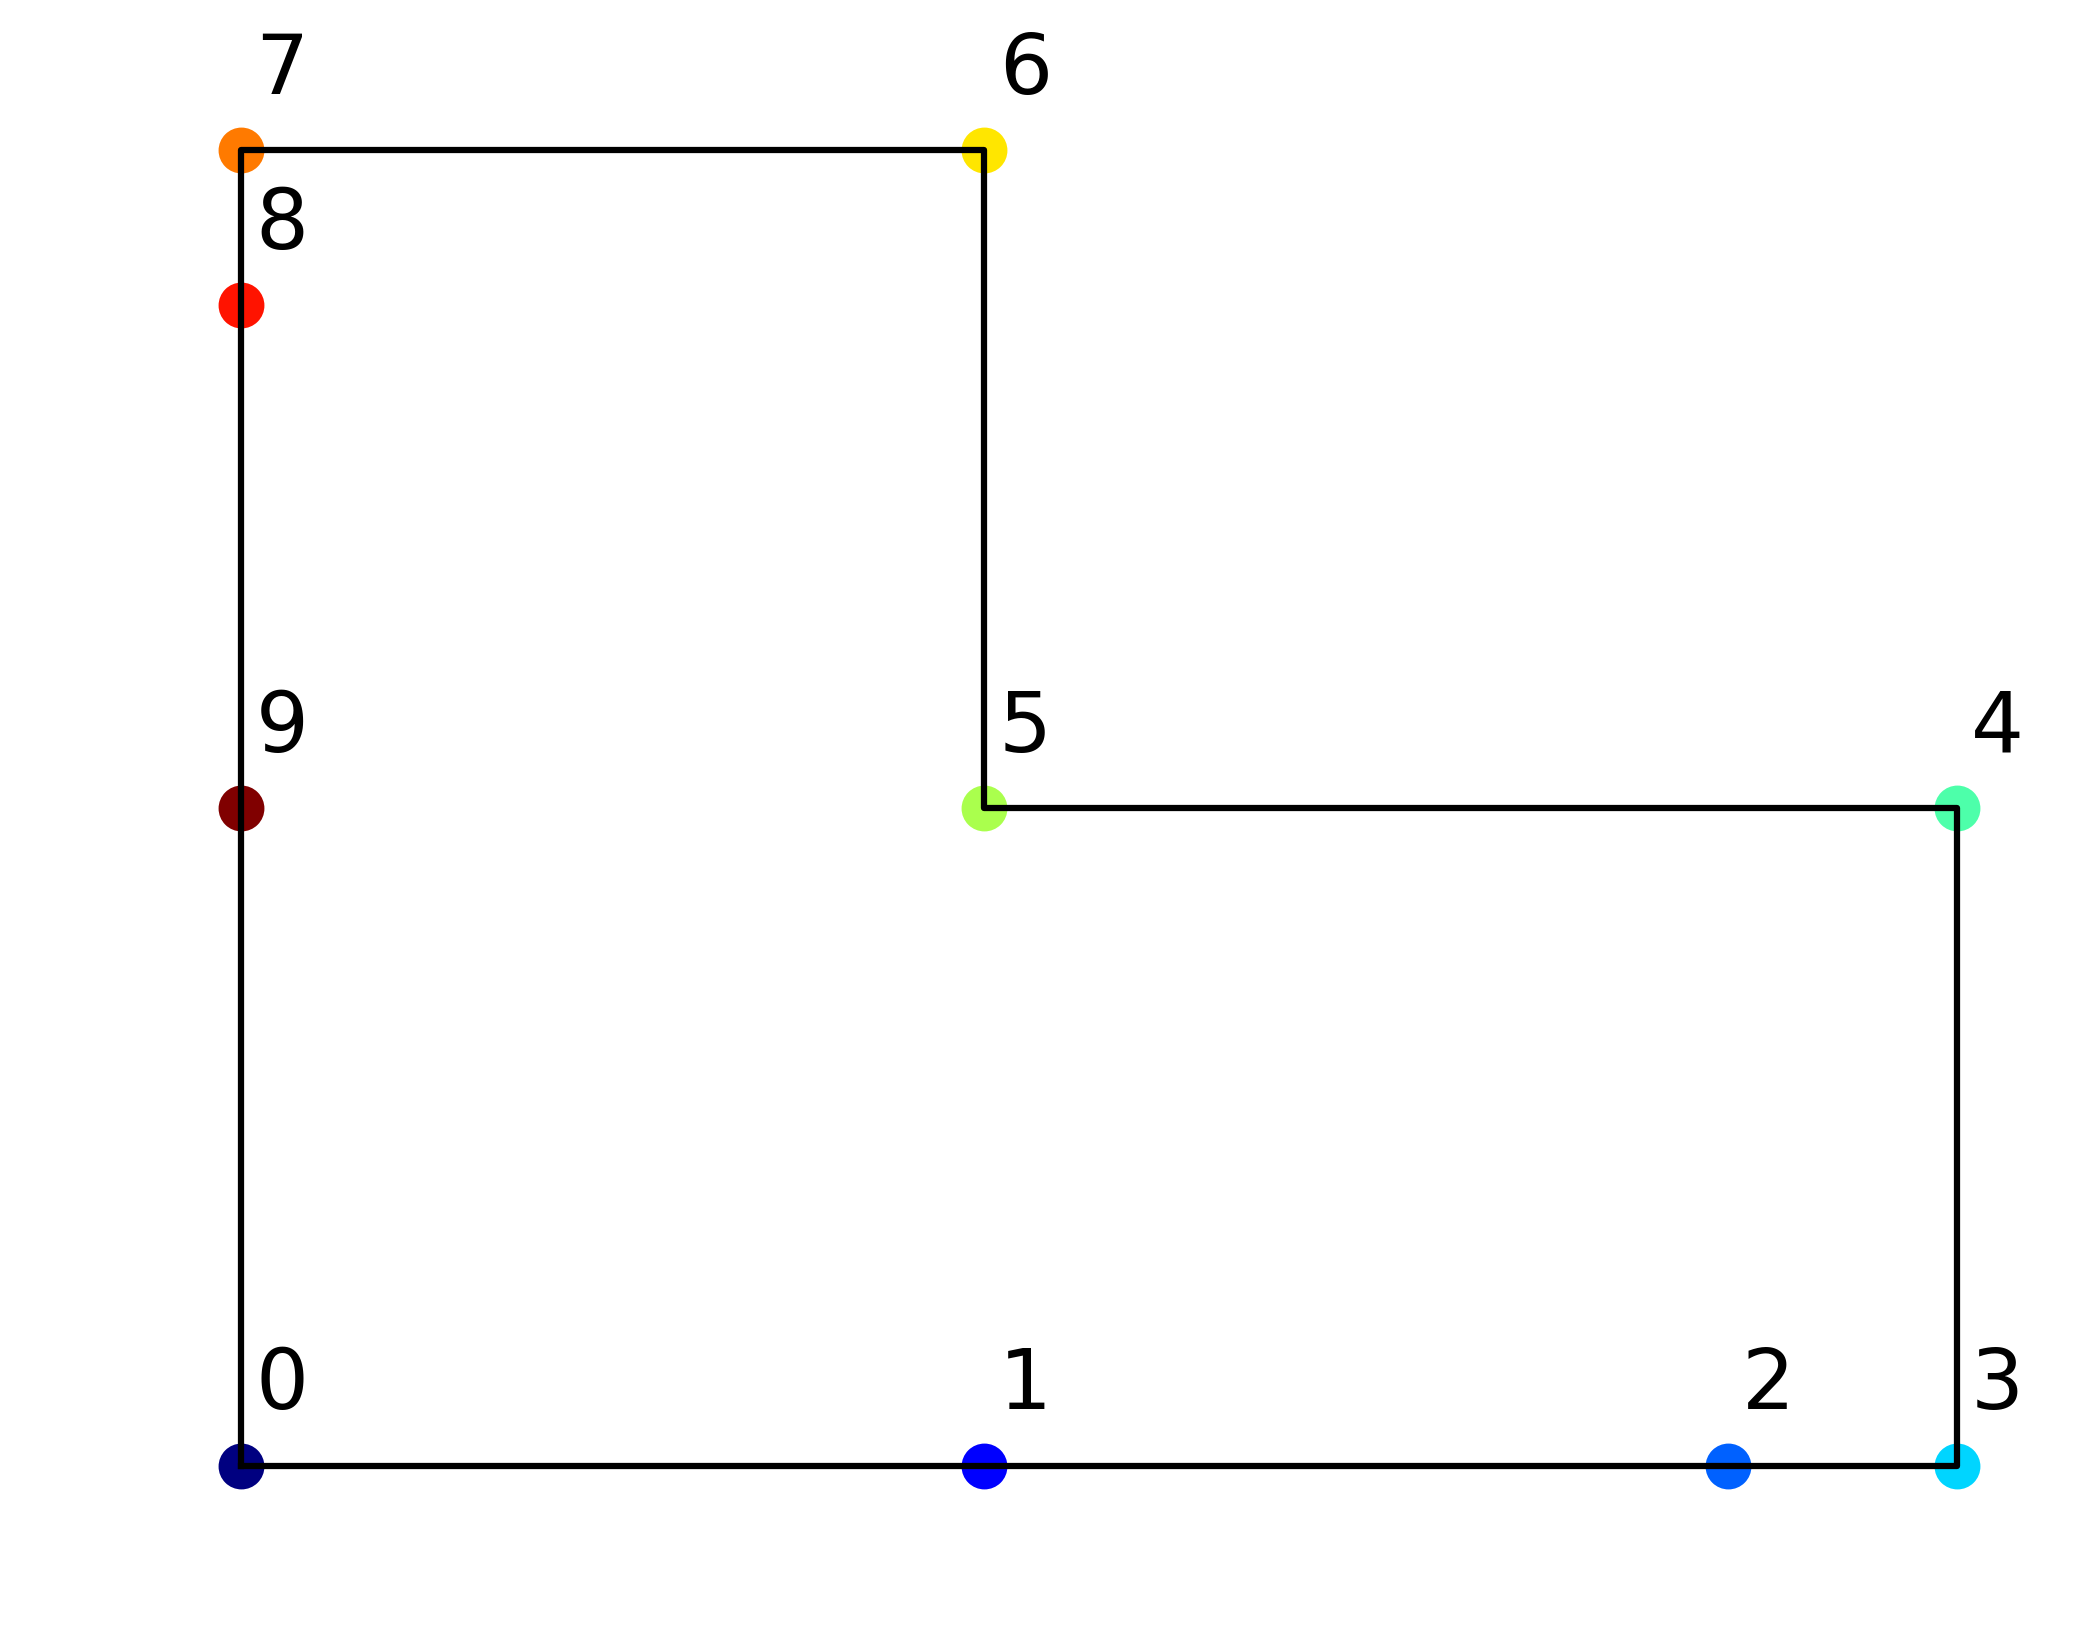
\includegraphics[width=\linewidth]{figures/L_poly.png}
\end{subfigure}%
\begin{subfigure}{0.5\textwidth}
\centering
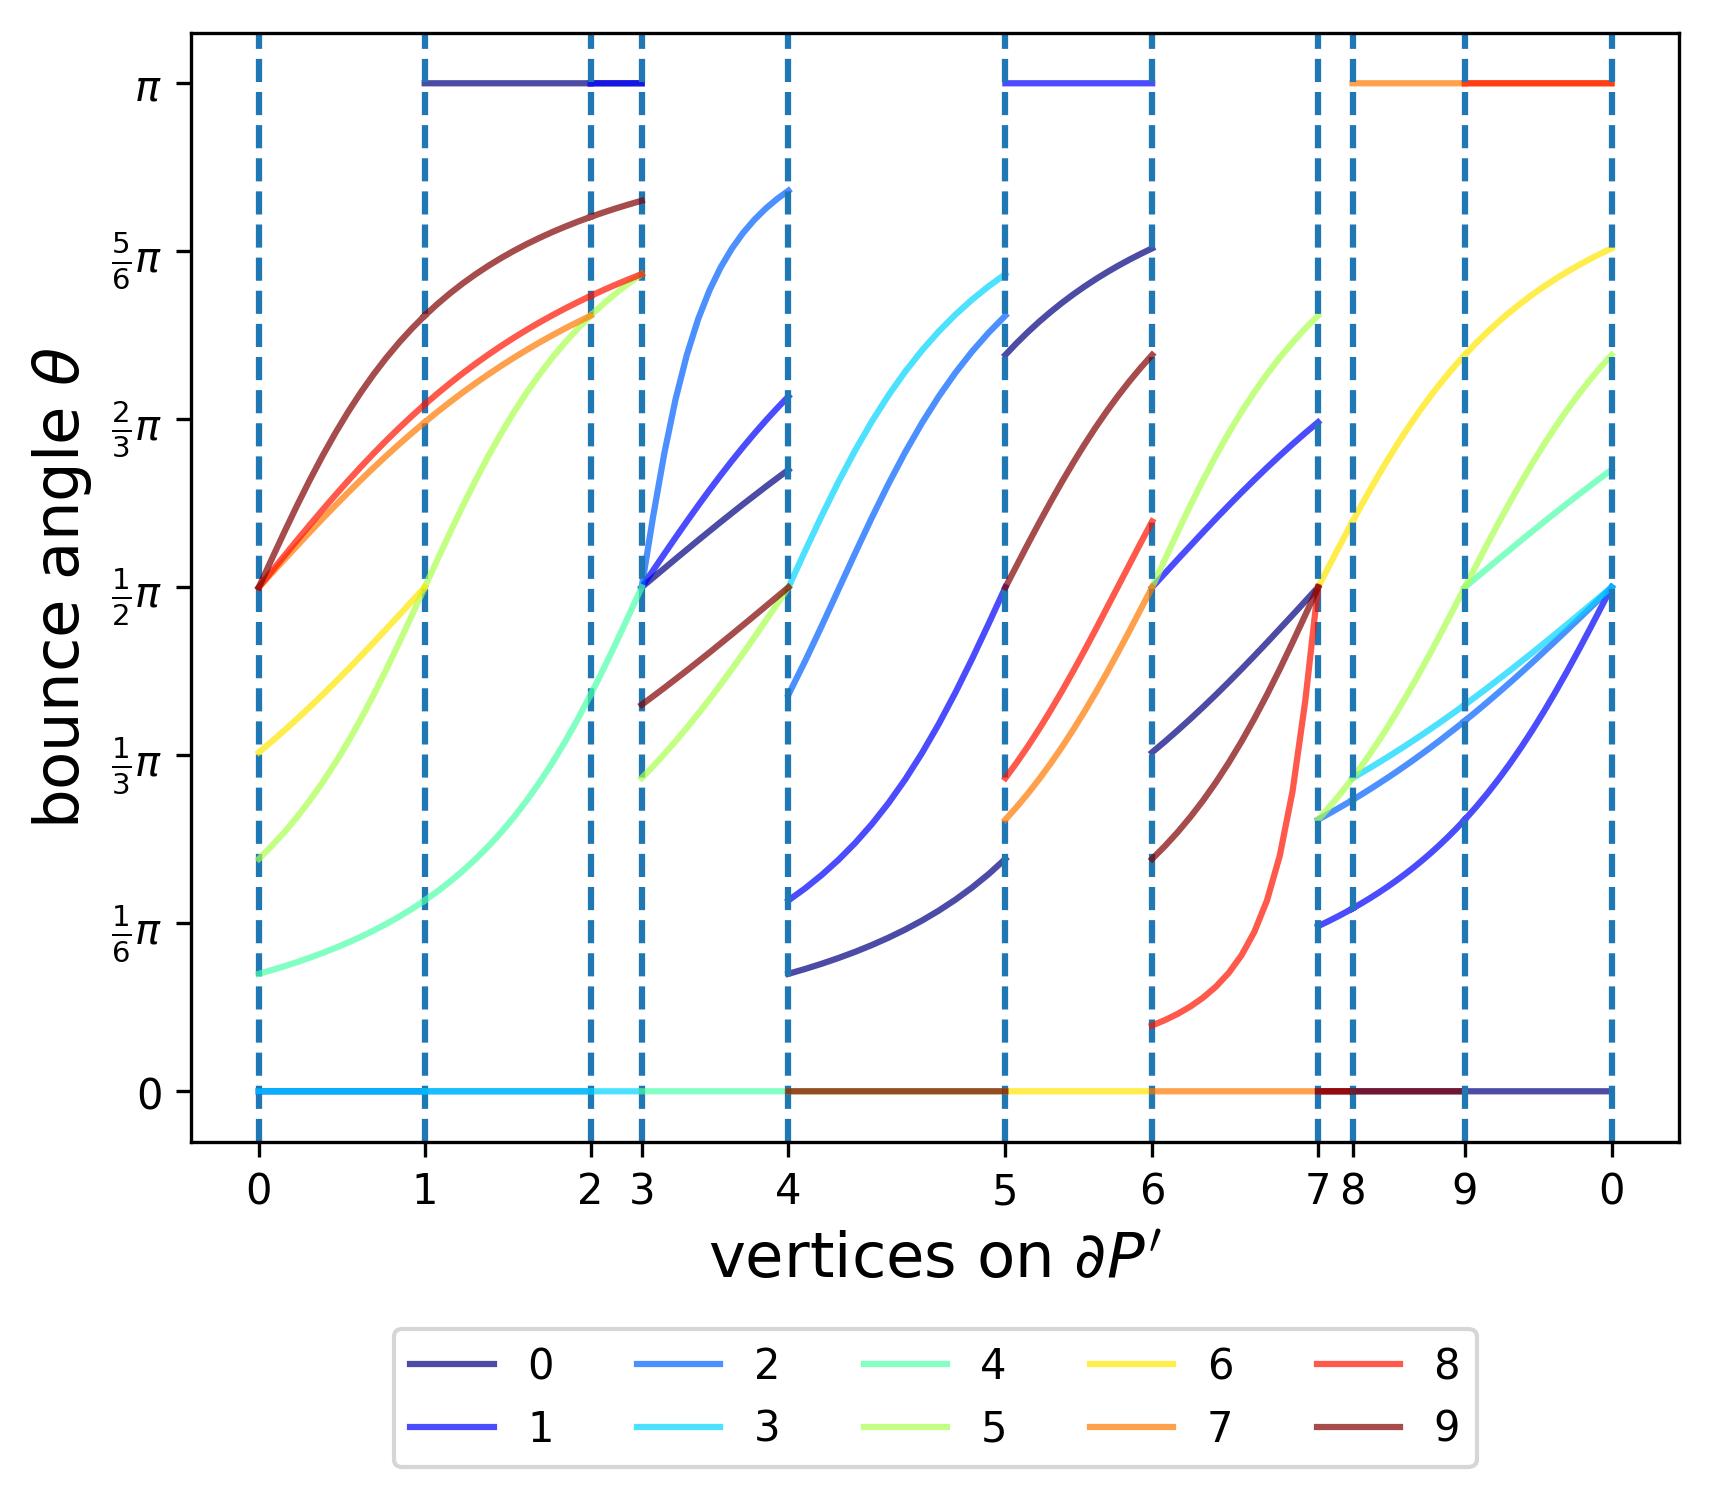
\includegraphics[width=\linewidth]{figures/L_diagram.png}
\end{subfigure}
\caption{A partitioned polygon and its corresponding bounce visibility diagram. }
\label{fig:diagram}
\end{figure}

The bounce visibility diagram gives us some visual insight into the structure of
the problem. First, it shows our motivation for the specific partitioning we
have chosen: at each inserted vertex (1, 2, 8, and 9 in Figure
\ref{fig:diagram}), another vertex appears or disappears from view. Of course, such
transitions also occur at the original vertices of $P$. Thus, the partition induced by the
vertices of $P$ and our inserted partial local sequences captures all
combinatorial changes in the visible vertices.

Additionally, this diagram gives us some insight into types of possible
segment-to-segment transitions under ranges of departure angles. 
For example, slicing the diagram vertically at a specific $s \in \partial P'$
produces a list of vertices visible from that point on the boundary (the
combinatorial visibility vector) \cite{suri2008simple}. The vertical dotted
lines, vertices of $P'$, are the exact points at which the combinatorial visibility
vector (cvv) changes. Within a segment $(v_i, v_{i+1})$, if two successive elements of the cvv are 
adjacent vertices, then \emph{some} transition exists from
$(v_i, v_{i+1})$ to a point on the edge between those vertices.

If for a segment $(v_i, v_{i+1})$, if there is an interval of $\theta$ such that
no vertex lines are crossed from left to right, this corresponds to our notion
of \emph{safe actions}; the robot can transition from segment to segment under
some amount of nondeterministic error in position and action.
For example, in
Figure \ref{fig:diagram}, we see that a band of intervals exists at the top and
bottom of the diagram with no ``crossings" as you move from left to right
(moving the robot around $\partial P$). These bands correspond to the safe
actions to be formally described in Proposition \ref{prop:twosafe}.

%{\color{red} current diagram just shows lines where the visibility polygon at s
%changes combinatorial structure. In between the lines, we are not guaranteed
%that all transitions land on the same segment. Would need to do another
%iteration of partition algorithm to determine destination segments.}
%
%For example, in Figure \ref{fig:regular_pent_bvd} we can see that
%there are intervals of $\theta$ for which we can draw lines horizontally across
%the diagram without crossing the solid lines. If we can draw a horizontal line
%for $\theta$ from $v_i$ to $v_{i+1}$, all transitions $f(s,\theta)$
%for any $s \in v_i v_{i+1}$ will be mapped to points in a single segment in
%$P'$. If we can
%draw such lines across the entire diagram, this indicates that this property
%holds true for the entire polygon. We call such transitions \emph{safe
%actions}, since for a range of $\theta$, $f(s,\theta)$ maps from one equivalence
%class on the boundary to another without splitting the $s$-interval.



\begin{proposition} \label{prop:complexity}
The bounce visibility graph for a polygon with $n$ vertices has 
$O(n^2)$ vertices and $O(n^4)$ edges.
\end{proposition}

The proof of Proposition \ref{prop:complexity} is left to the Appendix.

%\begin{figure}
%
%\centering
%\begin{subfigure}{0.35\textwidth}
%\centering
%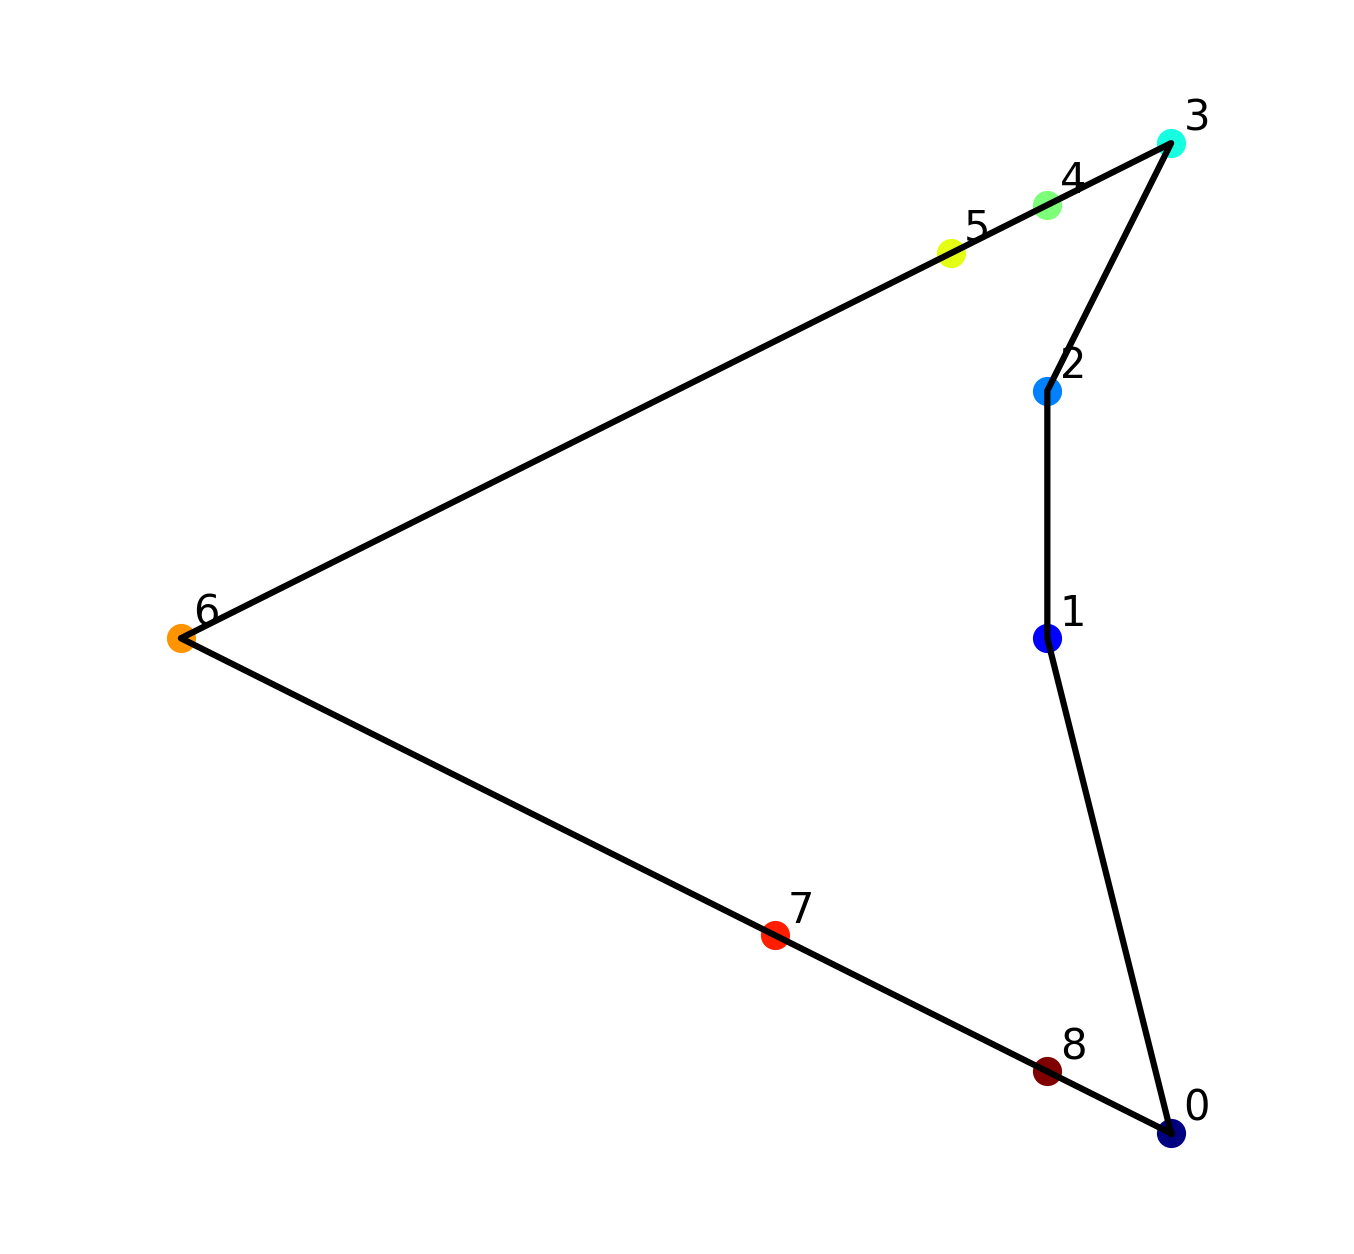
\includegraphics[width=\linewidth]{figures/color_pent.png}
%\captionof{figure}{\label{fig:color_pent}}
%\end{subfigure}%
%\begin{subfigure}{0.35\textwidth}
%\centering
%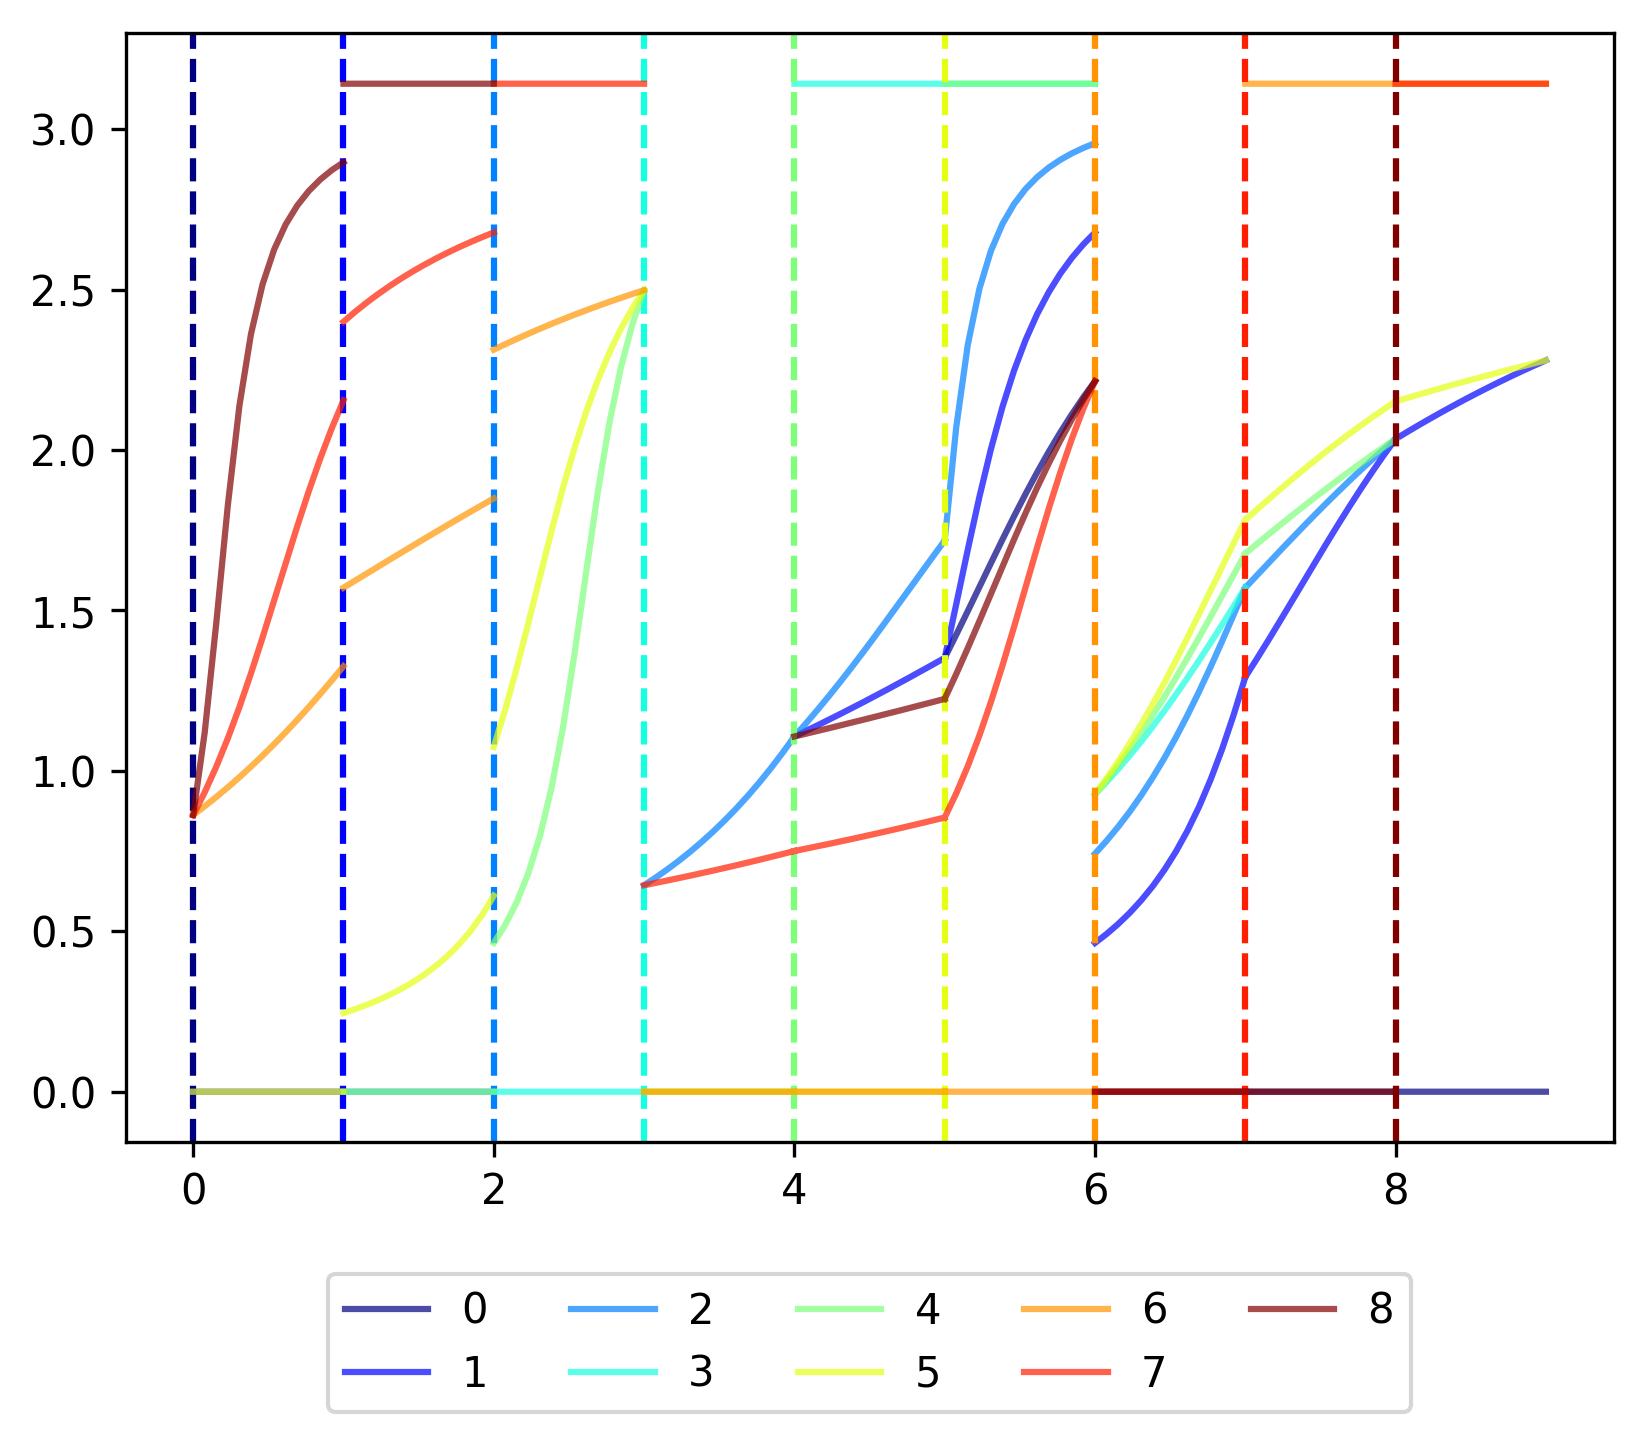
\includegraphics[width=\linewidth]{figures/bvd.png}
%\end{subfigure}
%\caption{A polygon and its corresponding bounce visibility diagram.}
%\label{fig:bvd}
%\end{figure}
%
\begin{figure}
\centering
\begin{subfigure}{0.5\textwidth}
\centering
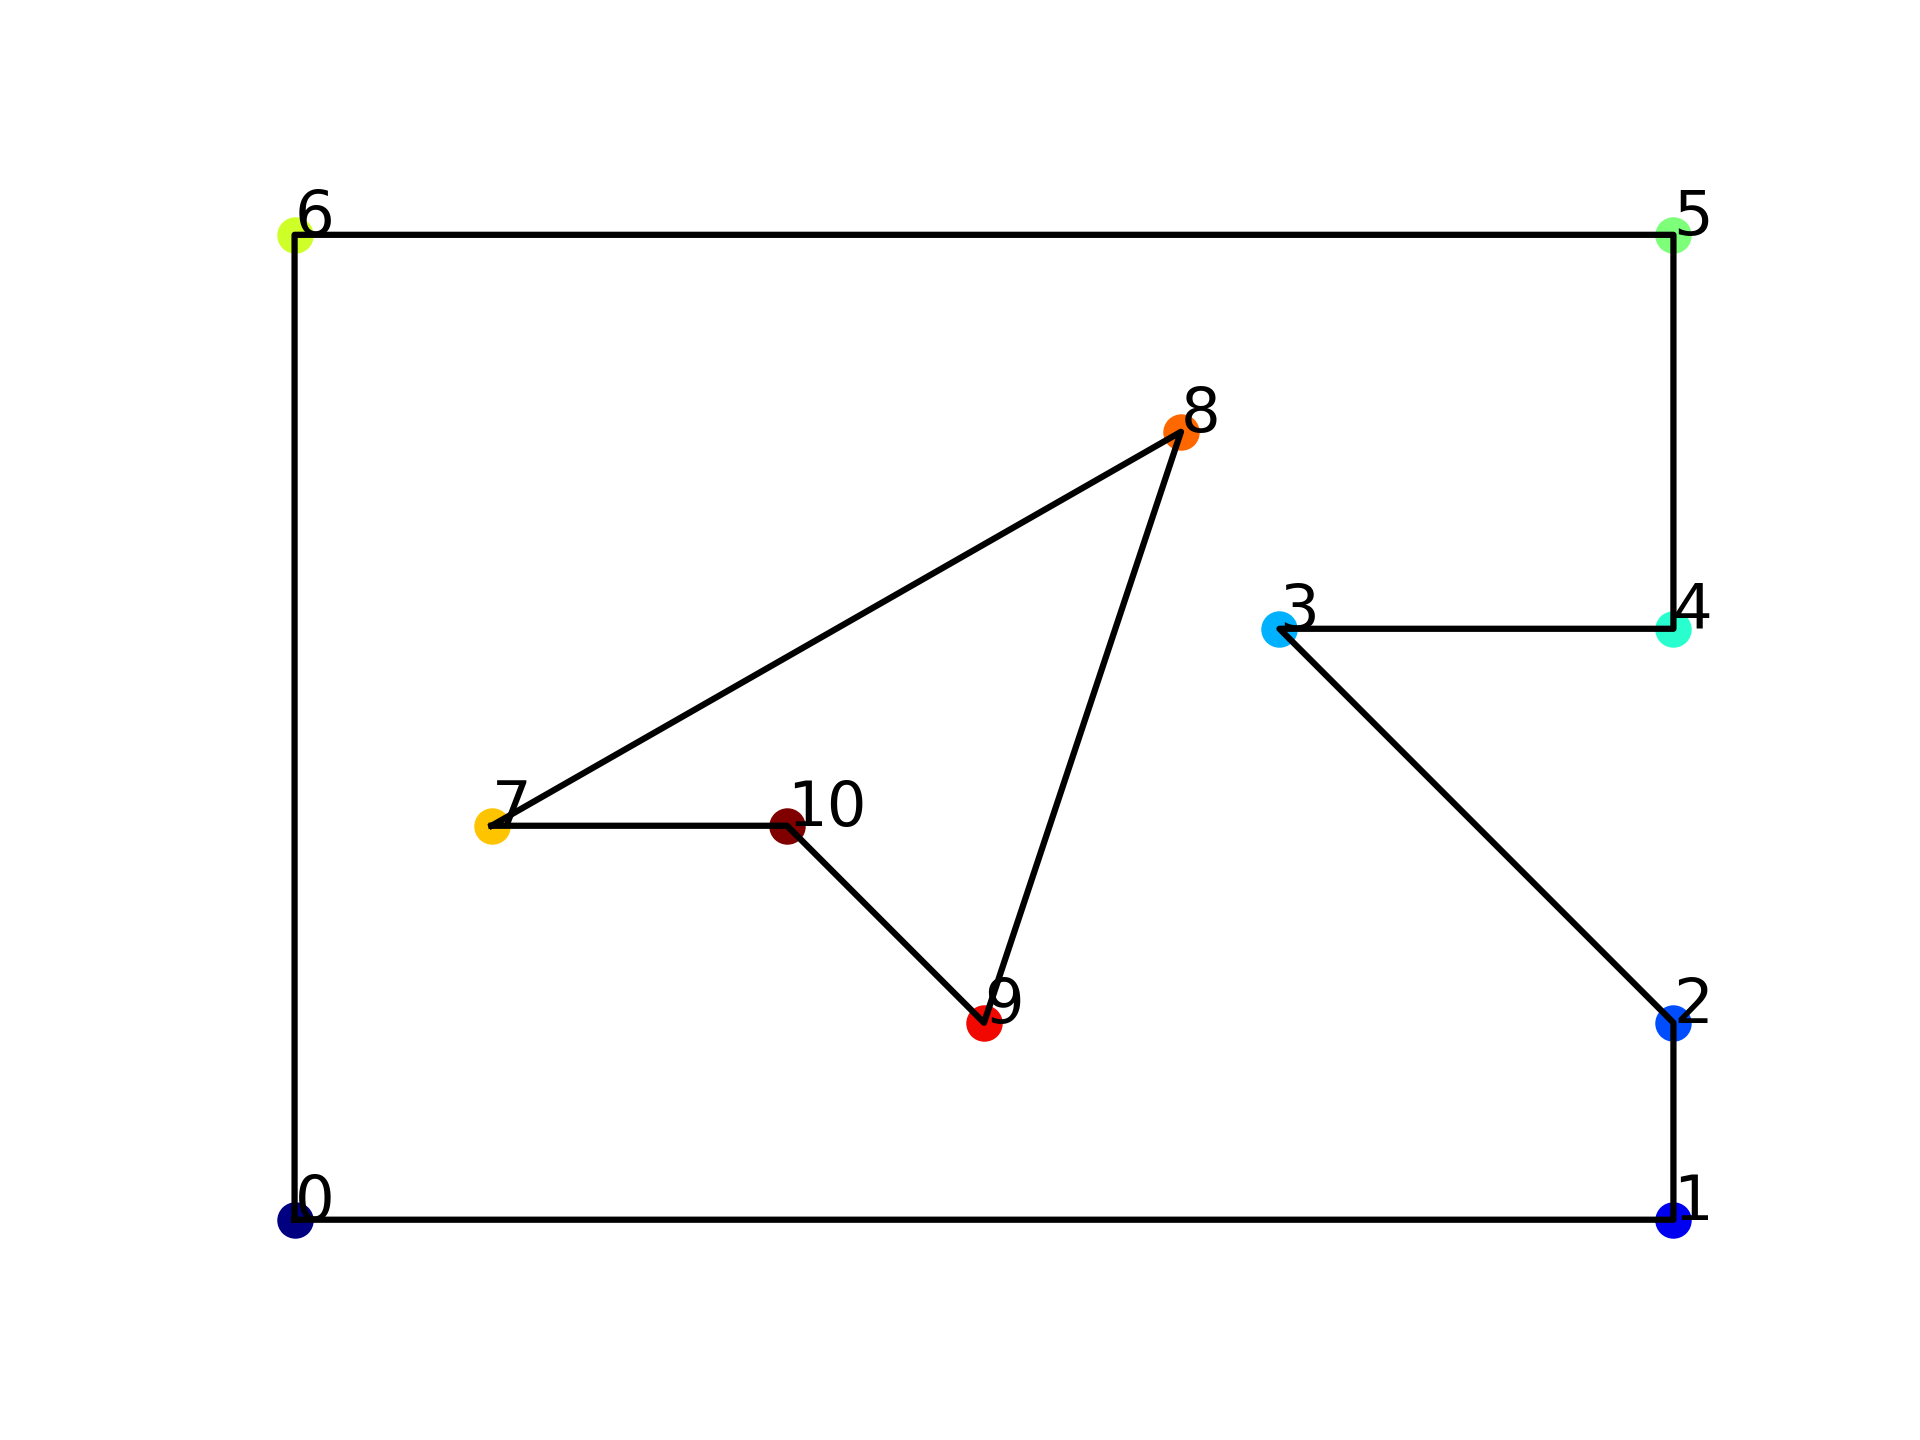
\includegraphics[width=0.5\linewidth]{figures/median_holes.png}
\centering
%\captionof{figure}{\label{fig:median_holes}}
\end{subfigure}%
\begin{subfigure}{0.5\textwidth}
\centering
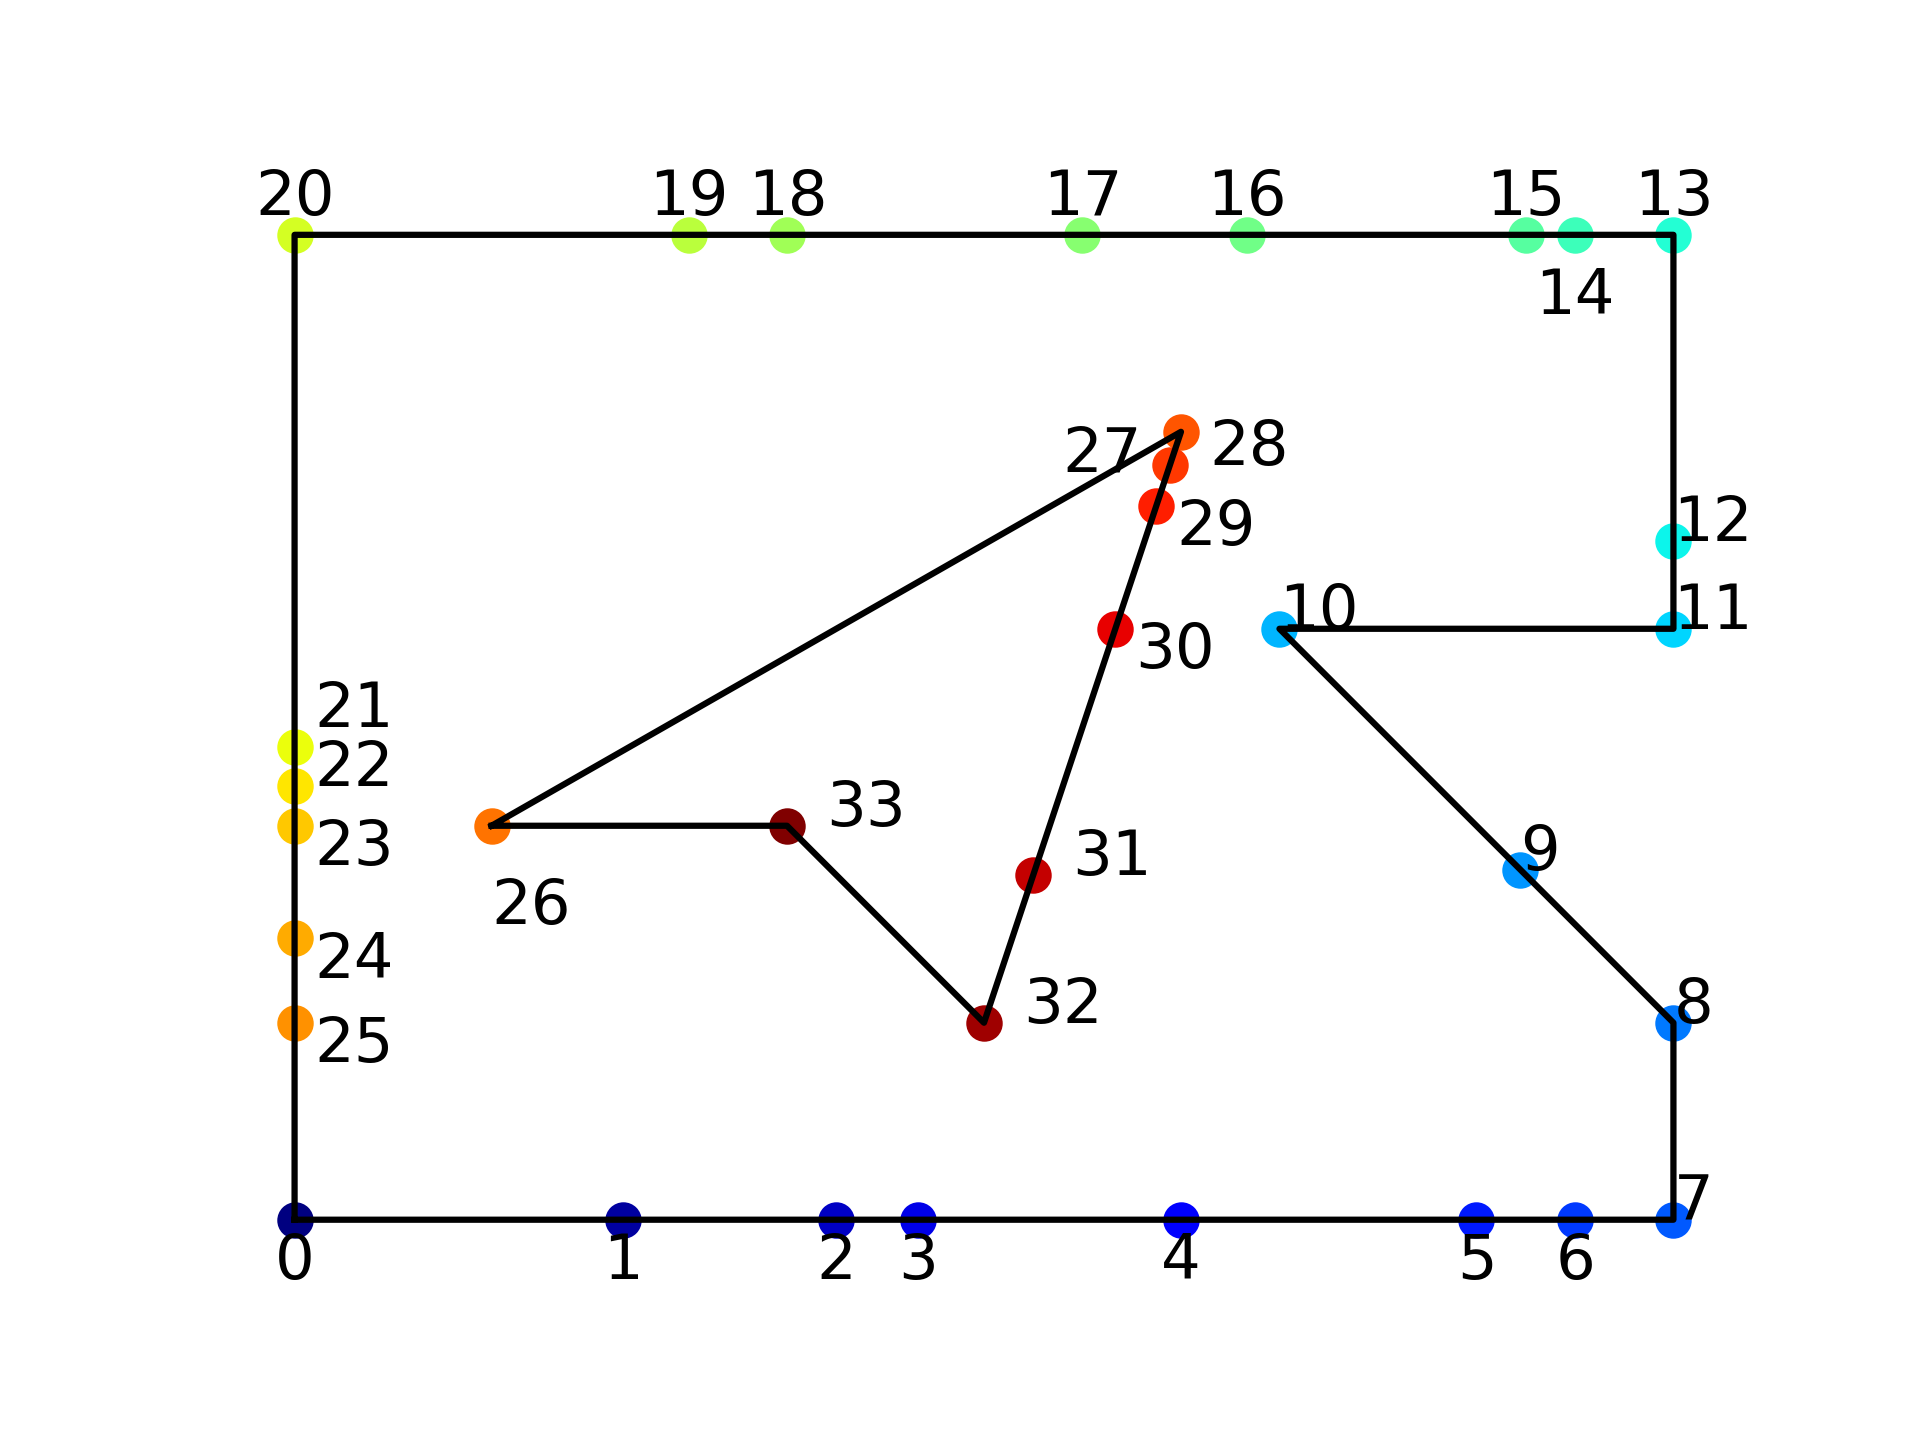
\includegraphics[width=0.5\linewidth]{figures/median_holes_inserted.png}
\centering
%\captionof{figure}{\label{fig:median_holes_inserted}}
\end{subfigure}
\begin{subfigure}{\textwidth}
\centering
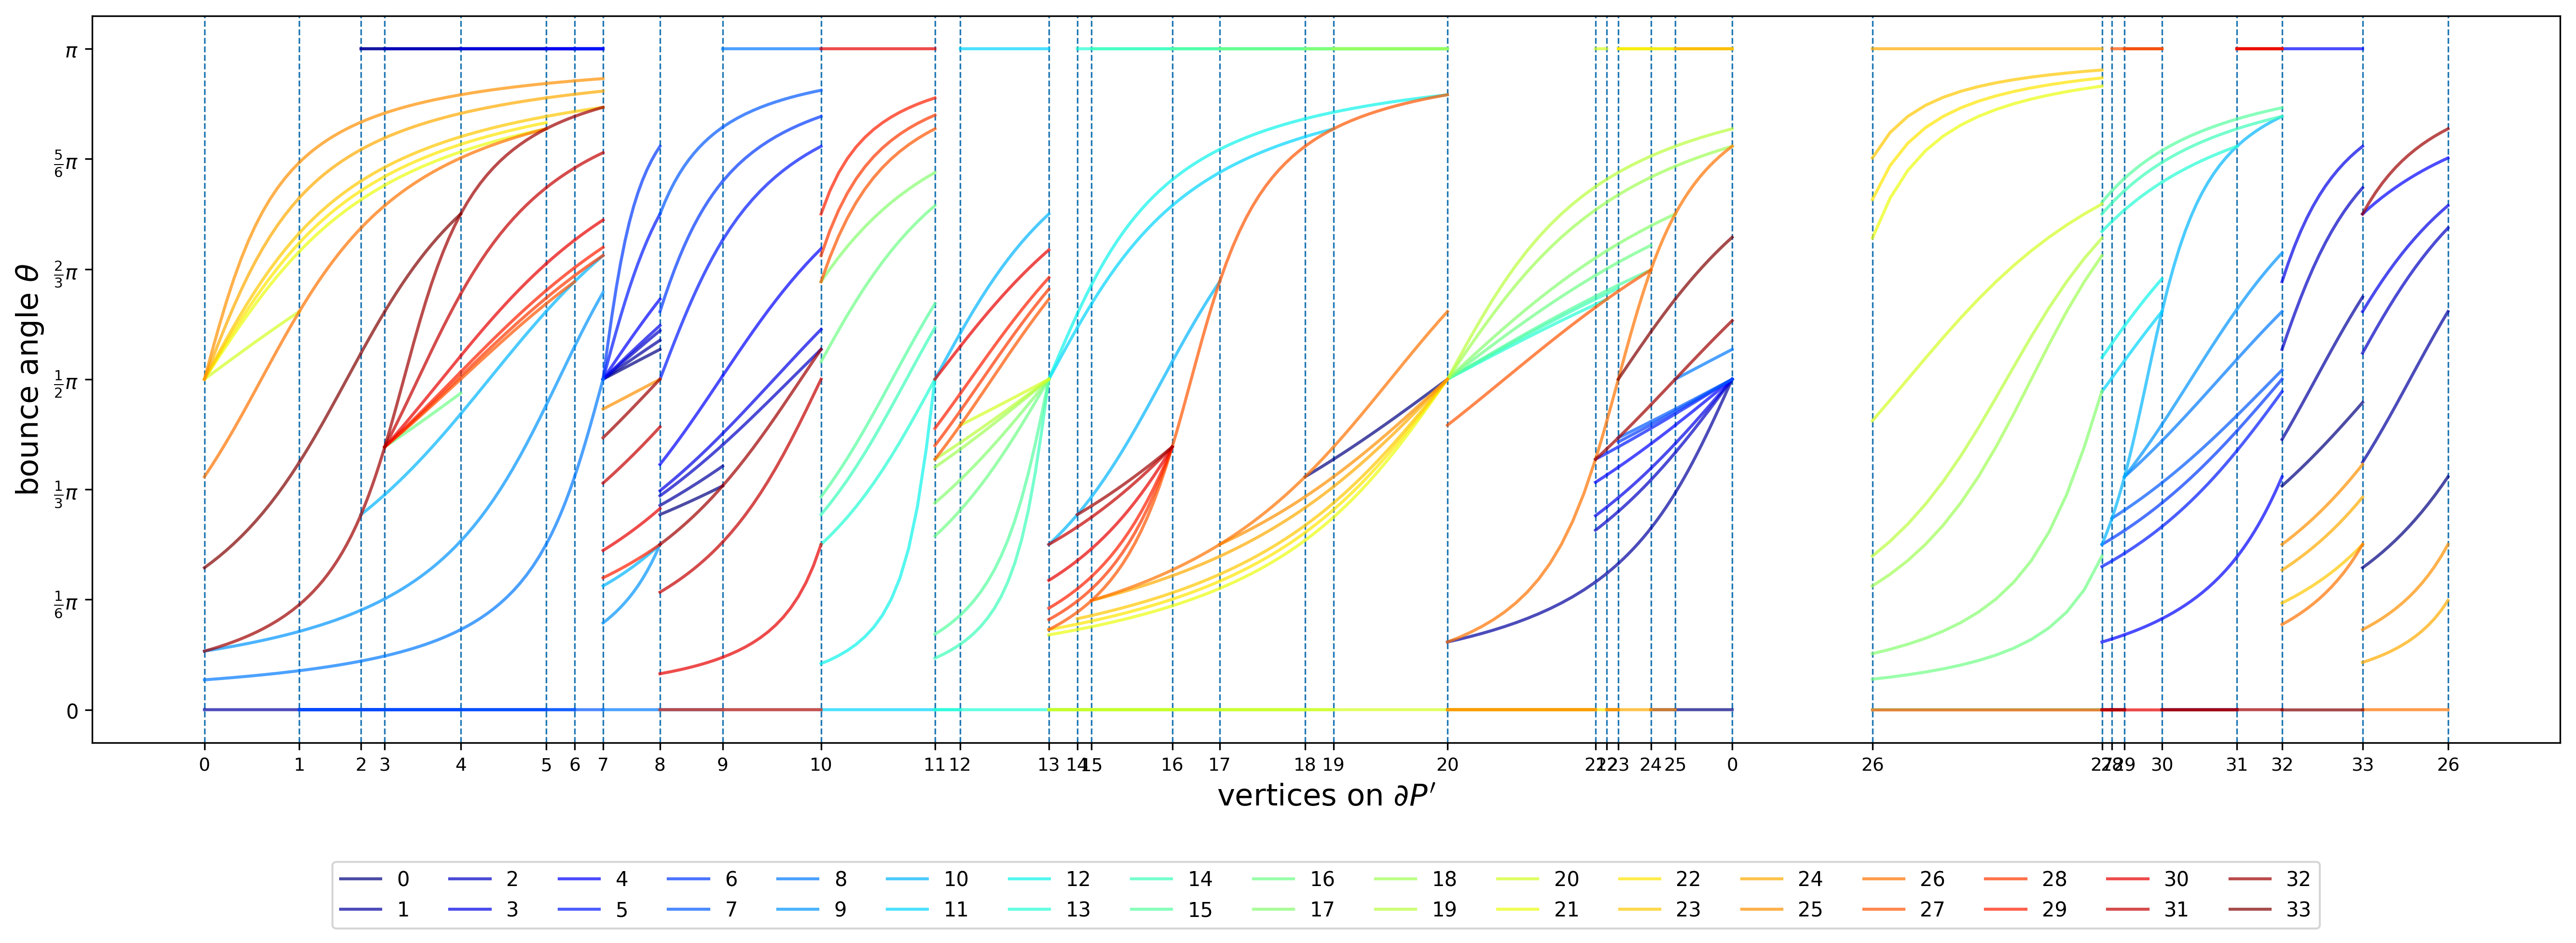
\includegraphics[width=\linewidth]{figures/median_holes_bvd_all_inserted.png}
\centering
%\captionof{figure}{\label{fig:median_holes_bvd_all_inserted}}
\end{subfigure}
\caption{An example bounce visibility diagram for a polygon with holes.}
\label{fig:bvd_holes}
\end{figure}

\section{Safe Actions} \label{sec:safe}

To characterize some families of paths, we will use the boundary
partition technique defined in Section \ref{sec:partition}, then define
\emph{safe actions} between segments in the partition that are
guaranteed to transition to the same edge from anywhere in the
originating edge. Such actions define transitions which keep the
robot state in one partition under nondeterministic actions.

\begin{definition}
Two edges $e_i,e_j$ of a polygon are \textbf{entirely visible} to each other if
and only if every pair of points $s_i \in e_i$ and $s_j \in e_j$ are visible (the
shortest path between $s_i$ and $s_j$ lies entirely within $P$).
\end{definition}

\begin{definition} \label{def:sa}
A \textbf{safe action} from edge $e_i$ to edge $e_j$ in a polygon is an 
action $u$ such
that $f(s,u) \in e_j$ for any $s \in e_i$ and $u$ in some interval of actions
$\tilde{\theta} \subseteq (0,\pi)$.
\end{definition}

\begin{proposition} \label{prop:saferange}
Given two entirely visible line segments $e_i = (v_i, v_{i+1})$ and $e_j =
(v_j, v_{j+1})$ in $\partial P'$, if a safe action
exists from $e_i$ to $e_j$, the maximum interval of safe actions is $\bm{\tilde{\theta} = [\theta_r, \theta_l]}$ such
that $\theta_r = \pi - \angle v_j v_{i+1} v_i$ and $\theta_l = \angle v_{j+1}
v_i v_{i+1}$.
\end{proposition}

For full proof, see the appendix. The sketch of the proof is that if $\theta_r$
is smaller than $\theta_l$, every ray shot from $e_i$ at $\theta \in [\theta_r,
\theta_l]$ must intersect with $e_j$.

Note that this definition of a safe action is very similar to the definition of an interval of
safe actions from \cite{LewOKa13}; the main differences in approach are the
generation of boundary segments, methods of searching the resulting graph, and
how we generate constraints on robot uncertainty instead of assuming uncertainty
bounds are an input to the algorithm.

\begin{lemma}
If two edges in $\partial P'$ are entirely visible to each other, then there will be at least one safe
action between them.
\end{lemma}

See Appendix for proof.

\begin{corollary} \label{coro:neighbor}
If two edges in $\partial P'$ share a vertex that is not reflex, and the two
 edges are not collinear, then there exist safe actions
from one to the other in both directions.
\end{corollary}

\begin{proof}
See Figure \ref{fig:safe_action_1}.
\end{proof}

\begin{definition}
Given two entirely visible segments $e_i$ and $e_j$,
rotate frame such that $e_i$ is aligned with the $x-$axis with its normal pointing
along the positive $y-$axis, such that 
segment $e_j$ is above segment $e_i$. If the intersection of segment $e_i$ and
$e_j$ would be on the left of segment $e_i$, then call the transition from $e_i$ to $e_j$ a
\textbf{left
transition}; if the intersection would be on the right of segment $e_i$, then call the
transition a \textbf{right transition}.
\end{definition}

\begin{proposition} \label{prop:twosafe}
For every polygon $P$ and the resulting partitioned polygon $P'$ under Algorithm
\ref{algo:insert}, each edge $e \in P'$ has at least two safe actions which allow
transitions away from $e$.
\end{proposition}

\begin{proof}

Let $e_i = (v_i, v_{i+1})$. Consider right transitions from $e_i$ to some $e_k$,
where the safe action interval $\tilde{\theta} = (0, \theta_l)$ for some 
nonzero $\theta_l$. We will show that such a transition must exist. 

By Corollary \ref{coro:neighbor}, if an edge $e_i$ has an adjacent edge
$e_{i+1}$ which is not collinear or separated by a reflex angle, 
$e_k = e_{i+1}$ and a safe transition exists
between $e_i$ and $e_{i+1}$ with $\theta_l = \angle v_{i+2} v_i v_{i+1}$. 
See Figure \ref{fig:safe_action_1}.

If the adjacent edge is at a reflex angle, Algorithm 
\ref{algo:insert} will insert a vertex in line with $e_i$ on the closest visible
edge, forming edge $e_k$. If $v_i$ is an original
vertex of $P$, $e_k$ will be entirely visible from $e_i$, since Algorithm
\ref{algo:insert} will otherwise insert a point in $v_i$'s partial local
sequence.

If $v_i$ is itself inserted by Algorithm \ref{algo:insert}, $e_k$ will still be
entirely visible. There must be some original vertex of $P$
clockwise from $v_i$ and collinear with $e_i$, which would insert a vertex
visible to $e_i$ through Algorithm \ref{algo:insert} if there were any reflex vertices
blocking transitions to $e_k$.
See Figure \ref{fig:safe_action_3} for an example of the geometry.

If the adjacent edge $e_{i+1}$ is collinear with $e_i$, take the first
non-collinear edge and apply the above reasoning to find $e_k$.
All the same arguments extend symmetrically to left transitions, which will have
safe actions of the form $\tilde{\theta} = [\theta_r, \pi)$. Thus, each edge will 
have two guaranteed safe actions leading away from it, in
some open interval of actions bordering the edge in each direction.

\qed
\end{proof}

\begin{figure}
\centering
\begin{subfigure}{0.3\textwidth}
\centering
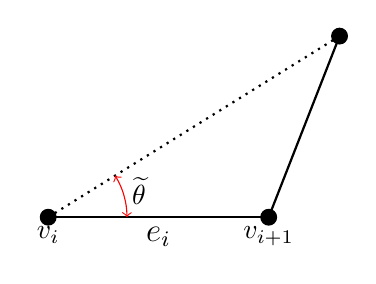
\begin{tikzpicture}
  \coordinate (A) at (-4, -0.8);
  \node at (A) [below] {$v_i$};
  \coordinate (B) at (-1.2, -0.8);
  \node at (B) [below] {$v_{i+1}$};
  \coordinate (C) at (-0.3, 1.5);
  \draw [fill] (A) circle [radius=0.1];
  \draw [fill] (B) circle [radius=0.1];
  \draw [fill] (C) circle [radius=0.1];
  \draw [thick](A) -- (B) node [midway, below, font = \large] {$e_i$};
  \draw [thick](B) -- (C);
  \draw[thick, dotted] (A) -- (C);
  \draw pic["$\widetilde{\theta}$",draw=red,<->,angle eccentricity=1.2,angle radius=1cm] {angle=B--A--C};
\end{tikzpicture}
\captionof{figure}{\label{fig:safe_action_1}}
\end{subfigure}%
%\begin{subfigure}{0.3\textwidth}
%\centering
%\begin{tikzpicture}
%  \coordinate (A) at (-3, -4);
%  \node at (A) [below] {$v_i$};
%  \coordinate (B) at (-0.1, -4);
%  \coordinate (C) at (0.8, -1.8);
%  \coordinate (D) at (-1.3, -4);
%  \coordinate (E) at (-1.1, -4.9);
%  \coordinate (F) at (-0.5, -4.9);
%  \coordinate (G) at (-1.9, -4);
%  \node at (G) [below] {$v_{i+1}$};
%  \draw [fill] (A) circle [radius=0.1];
%  \draw [fill] (B) circle [radius=0.1];
%  \draw [fill] (C) circle [radius=0.1];
%  \draw [fill] (D) circle [radius=0.1];
%  \draw [fill] (E) circle [radius=0.1];
%  \draw [fill] (F) circle [radius=0.1];
%  \draw [fill] (G) circle [radius=0.1];
%  \draw [thick](A) -- (G) node [midway, below, font = \large] {$e_i$};
%  \draw [thick](G) -- (D);
%  \draw [thick](D) -- (E);
%  \draw [thick](C) -- (F);
%  \draw[thick, dotted] (A) -- (C);
%  \draw[thick, dotted] (D) -- (B);
%  \draw pic["$\widetilde{\theta}$",draw=red,<->,angle eccentricity=0.8,angle radius=1cm] {angle=G--A--C};
%\end{tikzpicture}
%\centering
%\captionof{figure}{\label{fig:safe_action_2}}
%\end{subfigure}
\begin{subfigure}{0.3\textwidth}
\centering
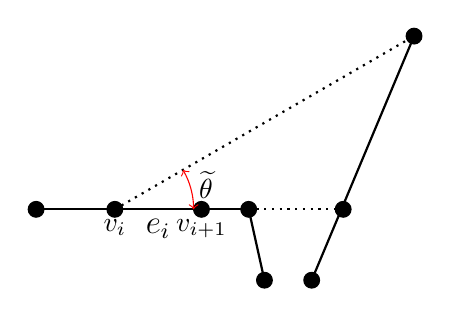
\begin{tikzpicture}
  \coordinate (A) at (-3, -4);
  \node at (A) [below] {$v_i$};
  \coordinate (B) at (-0.1, -4);
  \coordinate (C) at (0.8, -1.8);
  \coordinate (D) at (-1.3, -4);
  \coordinate (E) at (-1.1, -4.9);
  \coordinate (F) at (-0.5, -4.9);
  \coordinate (G) at (-1.9, -4);
  \coordinate (H) at (-4, -4);
  \node at (G) [below] {$v_{i+1}$};
  \draw [fill] (A) circle [radius=0.1];
  \draw [fill] (B) circle [radius=0.1];
  \draw [fill] (C) circle [radius=0.1];
  \draw [fill] (D) circle [radius=0.1];
  \draw [fill] (E) circle [radius=0.1];
  \draw [fill] (F) circle [radius=0.1];
  \draw [fill] (G) circle [radius=0.1];
  \draw [fill] (H) circle [radius=0.1];
  \draw [thick](A) -- (G) node [midway, below, font = \large] {$e_i$};
  \draw [thick](G) -- (D);
  \draw [thick](H) -- (A);
  \draw [thick](D) -- (E);
  \draw [thick](C) -- (F);
  \draw[thick, dotted] (A) -- (C);
  \draw[thick, dotted] (D) -- (B);
  \draw pic["$\widetilde{\theta}$",draw=red,<->,angle eccentricity=1.2,angle radius=1cm] {angle=G--A--C};
\end{tikzpicture}
\centering
\captionof{figure}{\label{fig:safe_action_3}}
\end{subfigure}
\caption{Examples of two of the types of safe action intervals.}
\label{fig:two_safe_cases}
\end{figure}

%\begin{definition}
%We say that two robot trajectories are in the same \textbf{combinatorial family}
%if they have the same number of collisions, and the collisions at stage $k$
%occur in the same segment of $P'$, for all $k$. Additionally, each transition in
%the trajectory must be performed by a safe action.
%\end{definition}


%\begin{definition}\label{def:transition}
%For edge $e_{ij} \in E(G)$, for each point $x$ in the edge $i$, there 
%exists a range of angles $\tilde{\theta}$ such that $f(x,\theta) \in j$ for
%some $\theta \in \tilde{\theta}$.
%\end{definition}
%
%\begin{proof}
%By construction, edge $e_{ij}$ exists if and only if there is a point $x$ on the (open)
%segment $i$ and a point $y$ on the (open) segment $j$ such that $x$ and $y$ are
%visible to each other. Since $y$ is in the open segment, there will always be some $\epsilon$-neighborhood around
%$y$ which is also visible from $x$, and the endpoints of this
%$\epsilon$-neighborhood define a range of angles at which the robot may leave
%$x$ and arrive on segment $j$.
%
%This angle range can be constructed through simple trigonometry for a
%given point and target segment.
%\end{proof}



\section{Dynamical Properties of Paths}

%Many tasks required of mobile robots can be specified in terms of properties of
%the path the robot takes through space. \emph{Navigation} requires a path that
%begins and ends in specified regions; \emph{patrolling} requires a repeatable
%path that satisfies some coverage criterion; \emph{localization} requires a path
%which reduces uncertainty in the robot's position.

Our motion strategy allows us to disregard the robot's motion in the interior of
$P$. Instead, the robot's state is an interval 
along the boundary $\partial P$, and we can formulate transitions as a discrete
dynamical system under the transition function $f$. The properties of this
dynamical system can be used to engineer paths corresponding to different robot
task requirements.

One such generally useful property of mapping functions is \emph{contraction}: 
when two points under the function always become closer together. We can use this property to control
uncertainty in the robot's position, and to engineer stable limit cycles in
Section \ref{sec:cycles}.

\begin{definition}
Let $\bm{\phi_{i,j}}$ be the interior angle between two edges $e_i, e_j \in \partial P$. 
\end{definition}

\begin{definition}

A function $g$ that maps a metric space $M$ to itself is a \textbf{contraction
mapping} if for all
$x, y \in M$, $\lvert g(x) - g(y) \rvert \leq c \lvert x-y \rvert$, and $0 \leq c < 1$.
\end{definition}

\begin{lemma} \label{lemma:angrange}
If the transition from segment $e_i$ to segment $e_j$ is a left transition, then the
transition function $f(x, \theta)$ between segments $e_i$ and $e_j$ is a contraction
mapping if and only if $\theta > \frac{\pi}{2}+\frac{\phi_{i, j}}{2}$;
if a right transition, the transition function $f(x, \theta)$ is a contraction mapping if
and only if $\theta < \frac{\pi}{2}-\frac{\phi_{i, j}}{2}$.
\end{lemma}

In our case, we will always take $M$ to be an interval in $\mathbb{R}$ and we
will use the L1 norm. The proof is a straightforward application of the law of sines, and is included
in the appendix.

\begin{corollary} \label{coro:existcontract}
For all pairs of adjacent 
segments with internal angle less than $\pi$,
there exists a range of actions for which $f$ is a contraction mapping.
\end{corollary}

\begin{definition}
The \textbf{contraction coefficient} of a transition between two
line segments is the ratio of the absolute distance between points before and after.
For a transition from $e_i$ to $e_j$ in $\partial P$, let the contraction
coefficient be denoted as $C(\theta, \phi_{i, j})$. 
For a left transition, $C(\theta, \phi_{i, j}) = | \frac{\sin(\theta)}{\sin(\theta - \phi_{i, j})} |$; 
for a right transition,  $C(\theta, \phi_{i, j}) = | \frac{\sin(\theta)}{\sin(\theta + \phi_{i, j})} |$.
\end{definition}

See the proof of Lemma \ref{lemma:angrange} in the appendix for derivation of
$C$. For a sequence of transitions $f_0, \ldots, f_k$, we can construct the overall
mapping from the domain of $f_0$ to the range of $f_k$ through function
composition. Since $f$ is a linear mapping, the contraction coefficient of a composition 
of multiple bounces can be determined by multiplying the contraction
coefficients of each bounce.

\begin{definition} \label{def:c}
Given a sequence of $m$ feasible transitions $F = \{f_0, f_1, \ldots, f_{m-1}\}$, at stage $k$ the robot 
will be located on edge $e(k)$ and will depart the edge with
action $\theta_k$; the contraction coefficient of the overall robot
trajectory $f_{m-1} \circ \ldots \circ f_0$ is $C(F) = \prod_{k=0}^{m-1} C(\theta_{k}, \phi_{e(k), e(k+1)})$.
\end{definition}

If $C(F) < 1$, the composition of $F$ is a contraction mapping. This is true even if some transition along
the way is not a
contraction mapping, since $C(F)$ is simply the ratio of distances
between points before and after the mapping is applied. Furthermore, the value
of $C(F)$ tells us the exact ratio by which the
size of the set of possible robot states has grown or shrank after $F$ is
executed.

\subsection{Cycles} \label{sec:cycles}

A contraction mapping that takes an interval back
to itself has a unique fixed point, by the Banach fixed point
theorem \cite{Granas2003}. Since the transition function of a path is the
composition of the individual transition functions, we can create a self-mapping 
by constructing a path which returns to its originating edge. A fixed
point of this mapping corresponds to a stable limit cycle.
Such trajectories in regular polygons were characterized in \cite{NilBecLav17}.
Here, we present a more general proof for the existence of limit cycles in all
convex polygons, with deterministic bounce rules.

\begin{definition}
$\phi_{P,min}$ is the smallest interior angle in a polygon $P$.
\end{definition}

\begin{theorem} \label{thm:convex}
For all convex polygons with $n$ edges, there exist constant fixed-angle bouncing
strategies which result in a period $n$ limit cycle regardless of the robot's start position.
\end{theorem}
\begin{proof}
See Figure \ref{fig:conv_cycle} in the Appendix for the geometric setup.

Without loss of generality, assume $\theta \in (0, \frac{\pi}{2}]$. The robot will always bounce
to the next adjacent edge if and only if
$\theta \in (0, \min_{i}(\angle v_{i+2}v_{i}v_{i+1}))$.

Suppose we have two start positions $s_1$ and $s_2$ on edge $e_0$ and a constant fixed bounce r
ule$b(\alpha, \theta) = \theta$.
At stage $k$, $s_1$ and $s_2$ will be located at $f^{k}(s_1,\theta)$ and
$f^{k}(s_2,\theta)$. 

By Definition \ref{def:c}, the distance between $s_1$ and $s_2$ changes after one orbit of the polygon by the
ratio $\frac{\lvert f^{n}(s_1, \theta) - f^{n}(s_2, \theta) \rvert}{ \lvert s_1
- s_2 \rvert } = \prod_{i = 0}^{n-1}
C(\theta, \phi_{i, i+1})$.

If this ratio is less than one, then $f^n(s,\theta)$ is a contraction
mapping from $e_0$ back to itself, and has a unique fixed point by the Banach fixed-point theorem
\cite{Granas2003}. By Lemma \ref{lemma:angrange}, this constraint is satisfied if  
$\theta < \frac{\pi}{2}-\frac{\phi_{i, i+1}}{2}$ for all $i$. We can guarantee that this
condition holds for the orbit by requiring

\begin{equation*}
\theta \in (0, \min(\min_{i = 0, 1, \dots, n-1}(\angle v_{i+2}v_{i}v_{i+1}),
\min_{i = 0, 1, \dots, n-1}(\frac{\pi}{2}-\frac{\phi_{i-1, i}}{2}))),
\end{equation*}

\noindent
in which case the fixed-angle bouncing strategy with $b(\alpha, \theta) = \theta$ leads to a convex
cycle which visits each edge of $P$ sequentially, regardless of the robot's start position.
The analysis follows similarly for orbits in the opposite direction.
\qed

\end{proof}

\begin{proposition} \label{prop:cycle}
For all points $s$ on the boundary of all polygons, a constant
fixed-angle controller exists which will cause the robot's trajectory to enter a
stable limit cycle.
\end{proposition}

\begin{proof}
First we observe that by Proposition \ref{prop:twosafe}, for every segment $e
\in \partial P'$, 
safe actions always exist
for two action intervals. These intervals are the ones bordering the segment itself:
by staying close enough to the boundary, the robot may guarantee a safe
transition. By Lemma \ref{lemma:angrange}, these safe actions will also
admit contraction mappings. Thus, we may choose a constant fixed-angle
controller such that it results in safe, contracting transitions from all
segments in $P'$. Since there are a finite number of segments in $P'$, this
controller must result in limit cycle from every point in $P$. If $s$ in on a
hole of the polygon, this procedure will cause the robot to leave the hole and
enter a cycle on the exterior boundary. \qed
\end{proof}

\section{Applications}

\subsection{Navigation}

Here, we define the \emph{navigation} task, which in our case will assume that
our robot has unavoidable uncertainty in its actuation. Thus, we wish to compute 
a strategy of \emph{nondeterministic bounce rules} guaranteed to take a robot
from any point in a starting set to some point in a goal set, as long as some
action in the bounce angle interval is successfully executed at each stage. 

\begin{definition}
\textbf{Navigation}:
Given a polygonal environment $P$, a convex starting set $S \subset \partial P$ of possible robot positions along the
environment boundary, and a convex goal set $G \subset \partial P$, determine a strategy $\pi$ which
will be guaranteed to take the robot from any point in $S$ to a point in $G$, or
determine that no such strategy exists.
\end{definition}

Using the formalisms built up so far, we can perform the navigation task as a
search over a discrete bounce visibility graph. Shortest paths in the graph 
will correspond to paths with the fewest number of bounces. It is important to
note that an arc $e_i \to e_k$ in the bounce visibility graph only implies that for each
point $x \in e_i$ there exists an action taking $x$ to some point in $e_k$. For
our navigation task, we require a {\em range} of angles which can take {\em any}
point in $e_i$ to a point on $e_k$, so we restrict the arcs of the bounce
visibility graph to those corresponding to safe actions only.

Many different
strategies for searching this graph could be defined; here, we will show how to
search for a constant fixed-angle bounce controller, where at every stage the
robot executes a fixed-angle bounce in the same range $\tilde{\theta}$. This is an
extension of the controllers analyzed in \cite{NilBecLav17} for regular polygons.

We define a few helper functions:

\begin{itemize}
\item \textsc{mkBVG}: Uses the visibility information generated in Algorithm
\ref{algo:insert} to generate the bounce visibility graph in $O(n^4)$ time.
\item \textsc{mkSafeBVG}: Using Definition \ref{def:sa} and Proposition \ref{prop:saferange}, we can create a \emph{safe roadmap}, $G_{safe}$,
        out of the bounce visibility graph by traversing all edges and removing edges with an 
        empty $\tilde{\theta}$, and labelling the remaining edges with the interval 
        of safe actions.
\item \textsc{SearchConstantFixedStrats}: performs breadth-first search from
start to goal, starting with $\tilde{\theta} = (0, \pi)$ and intersecting
$\tilde{\theta}$ with the safe action intervals along each path, terminating
when all start states reach a goal state at the same stage with overlapping
$\tilde{\theta}$ intervals.
\end{itemize}

\begin{algorithm}
\caption{\textsc{SafeConstantFixedNavigate}($P$, $S$, $G$, $k$)}
\label{algo:nav}
\hspace*{\algorithmicindent} \textbf{Input:} A polygon $P$, intervals $S$ and
$G$ in $\partial P$, and an integer bound $k$.\\
\hspace*{\algorithmicindent} \textbf{Output:} A strategy (list of bounce rules),
or a special value \textsc{None} if no strategy can be found.
\begin{algorithmic}[1]
\State $P' \gets$ \Call{PartitionPoly}{$P$}
\State $BVG \gets$ \Call{mkBVG}{$P'$}
\State $BVG_{safe} \gets$ \Call{mkSafeBVG}{$BVG$}
\State \textbf{return} \Call{SearchConstantFixedStrats}{$BVG_{safe}$, $S$, $G$, $k$}
\end{algorithmic}
\end{algorithm}


\begin{proposition}
There exist simple polygons such that under Algorithm \ref{algo:insert}, there
exist edges in the partitioned polygon $P'$ that are \textbf{not} reachable by 
a safe action from any other edge in $P'$.
\end{proposition}

\begin{proof}
See Figure \ref{fig:simple_bit} for an example in which the edge
counterclockwise from vertex 10 is not reachable via safe actions. Equivalently,
node 10 in $G_{safe}$ has no incoming arcs.

The only such segments will be
segments for which both endpoints are vertices inserted by Algorithm
\ref{algo:insert} or reflex vertices, since by Corollary \ref{coro:neighbor},
segments adjacent to non-reflex vertices of $P$ will be reachable by a safe
action. Thus, navigation using paths in $G_{safe}$ is not complete: we cannot
get everywhere safely, at least under this partitioning of $\partial P$.
\end{proof}

\begin{figure}
\centering
\begin{subfigure}{0.5\textwidth}
\centering
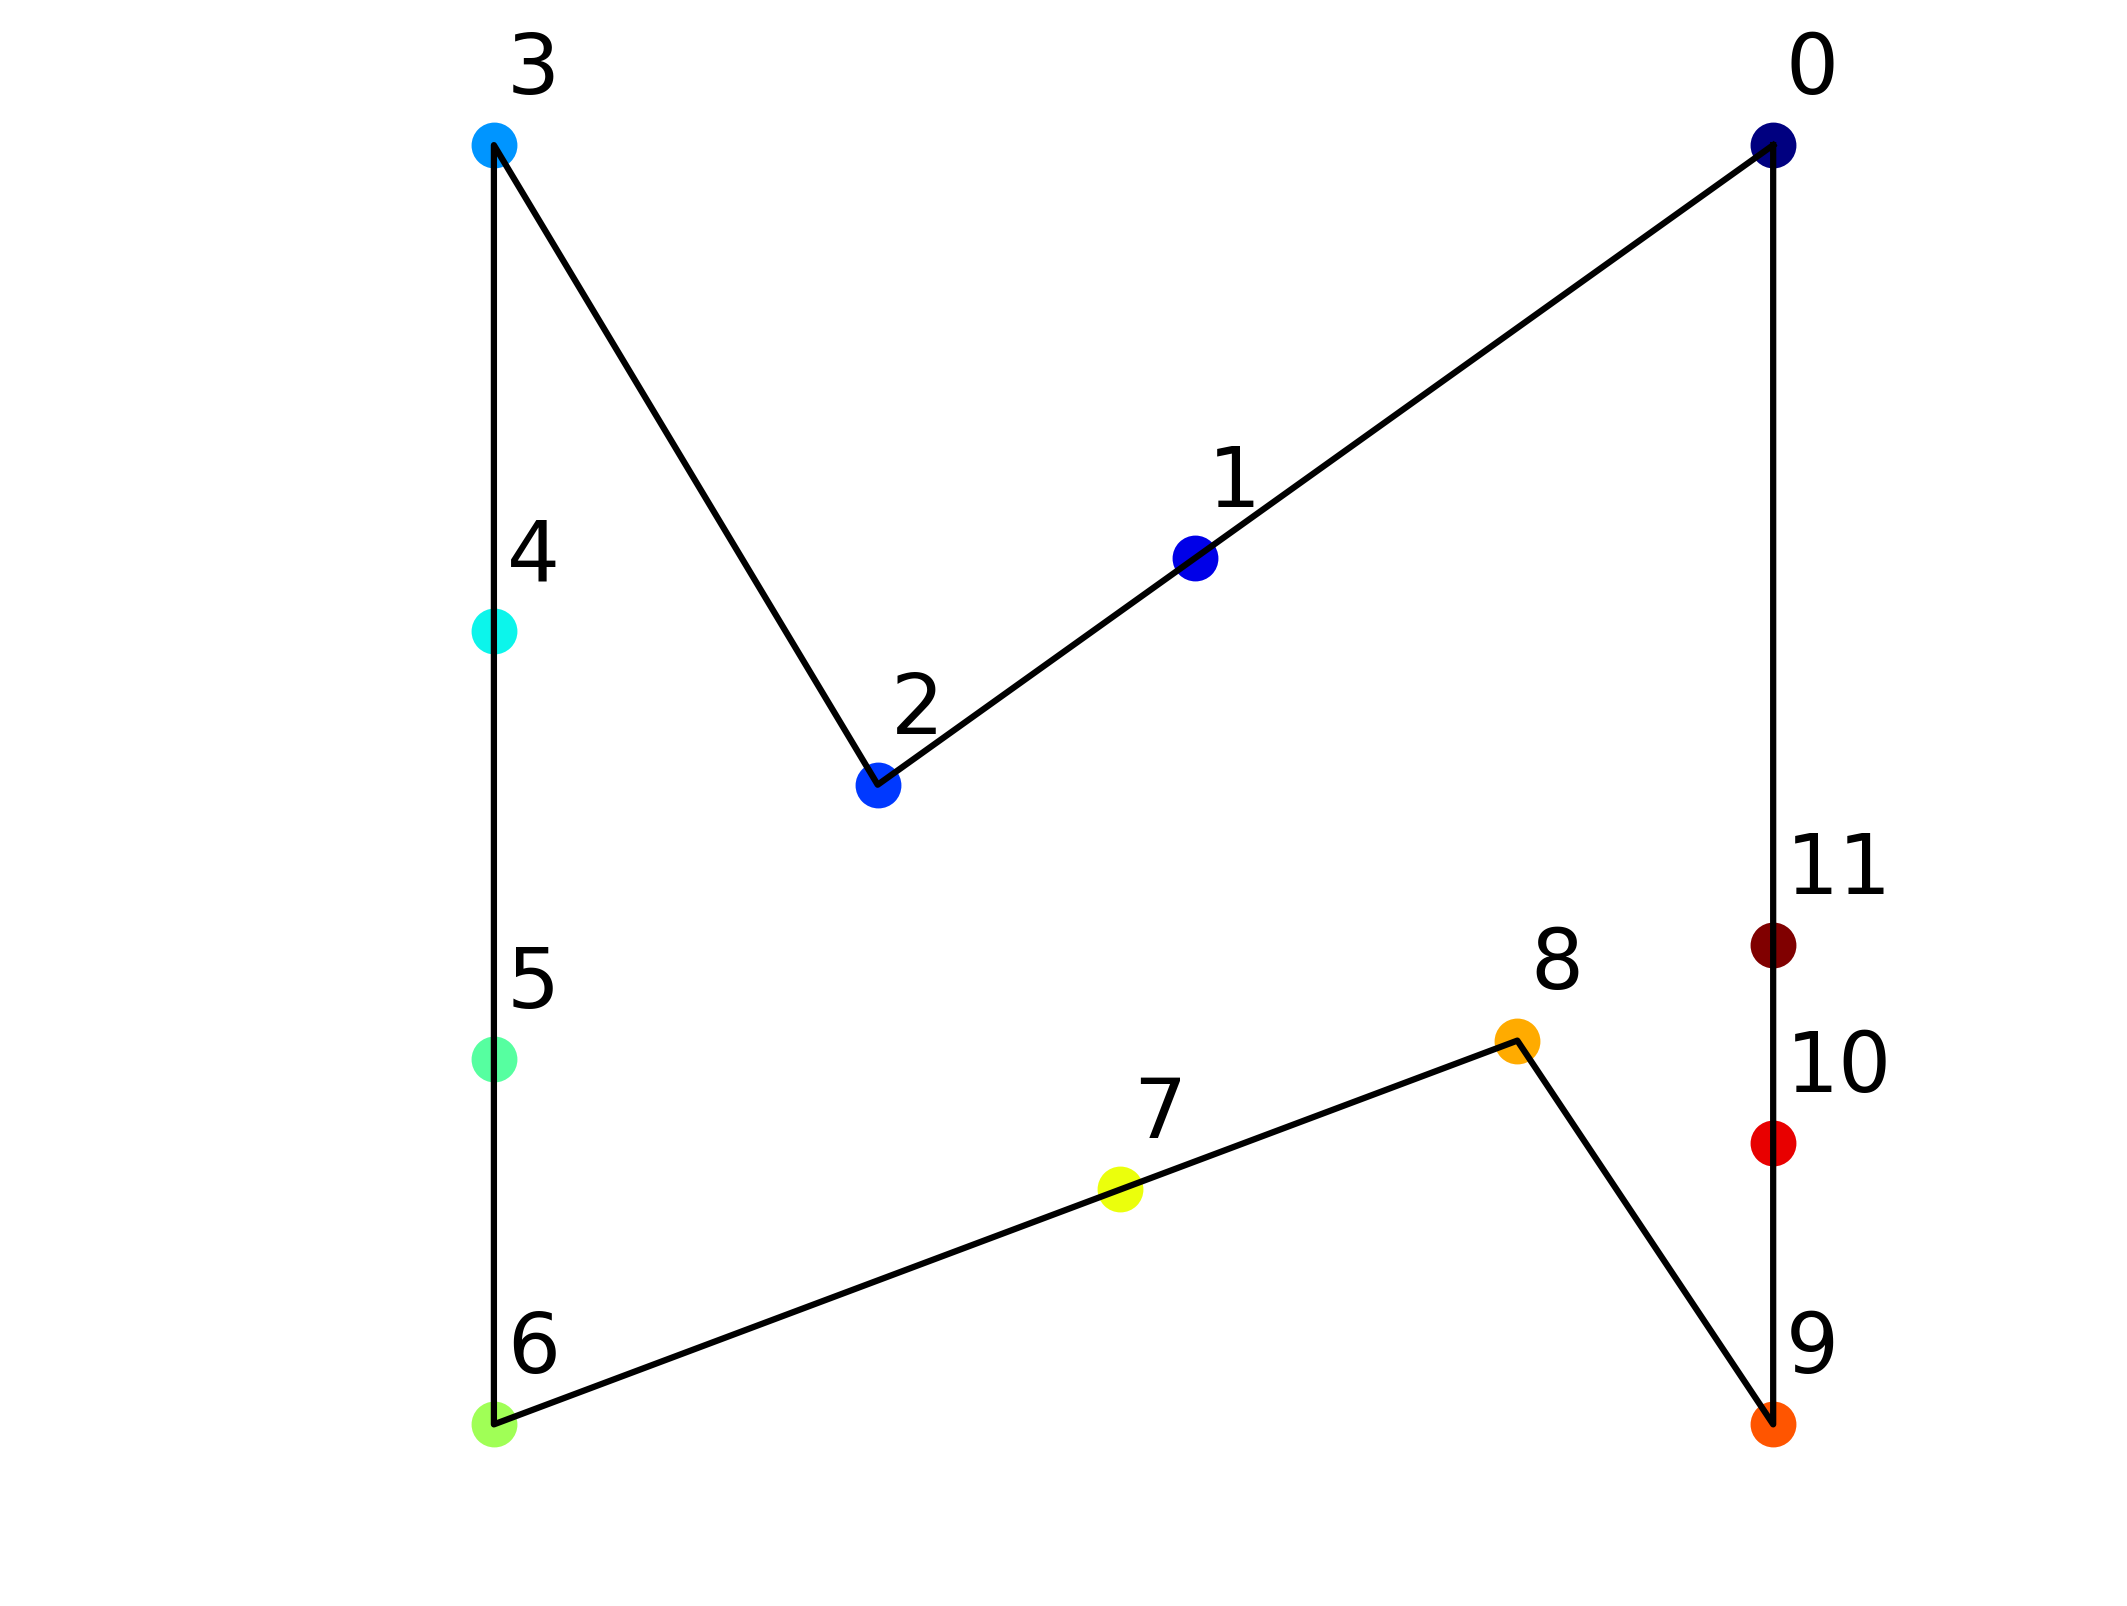
\includegraphics[width=\linewidth]{figures/simple_bit_inserted.png}
%\captionof{figure}{\label{fig:simple_bit_inserted}}
\end{subfigure}%
\begin{subfigure}{0.5\textwidth}
\centering
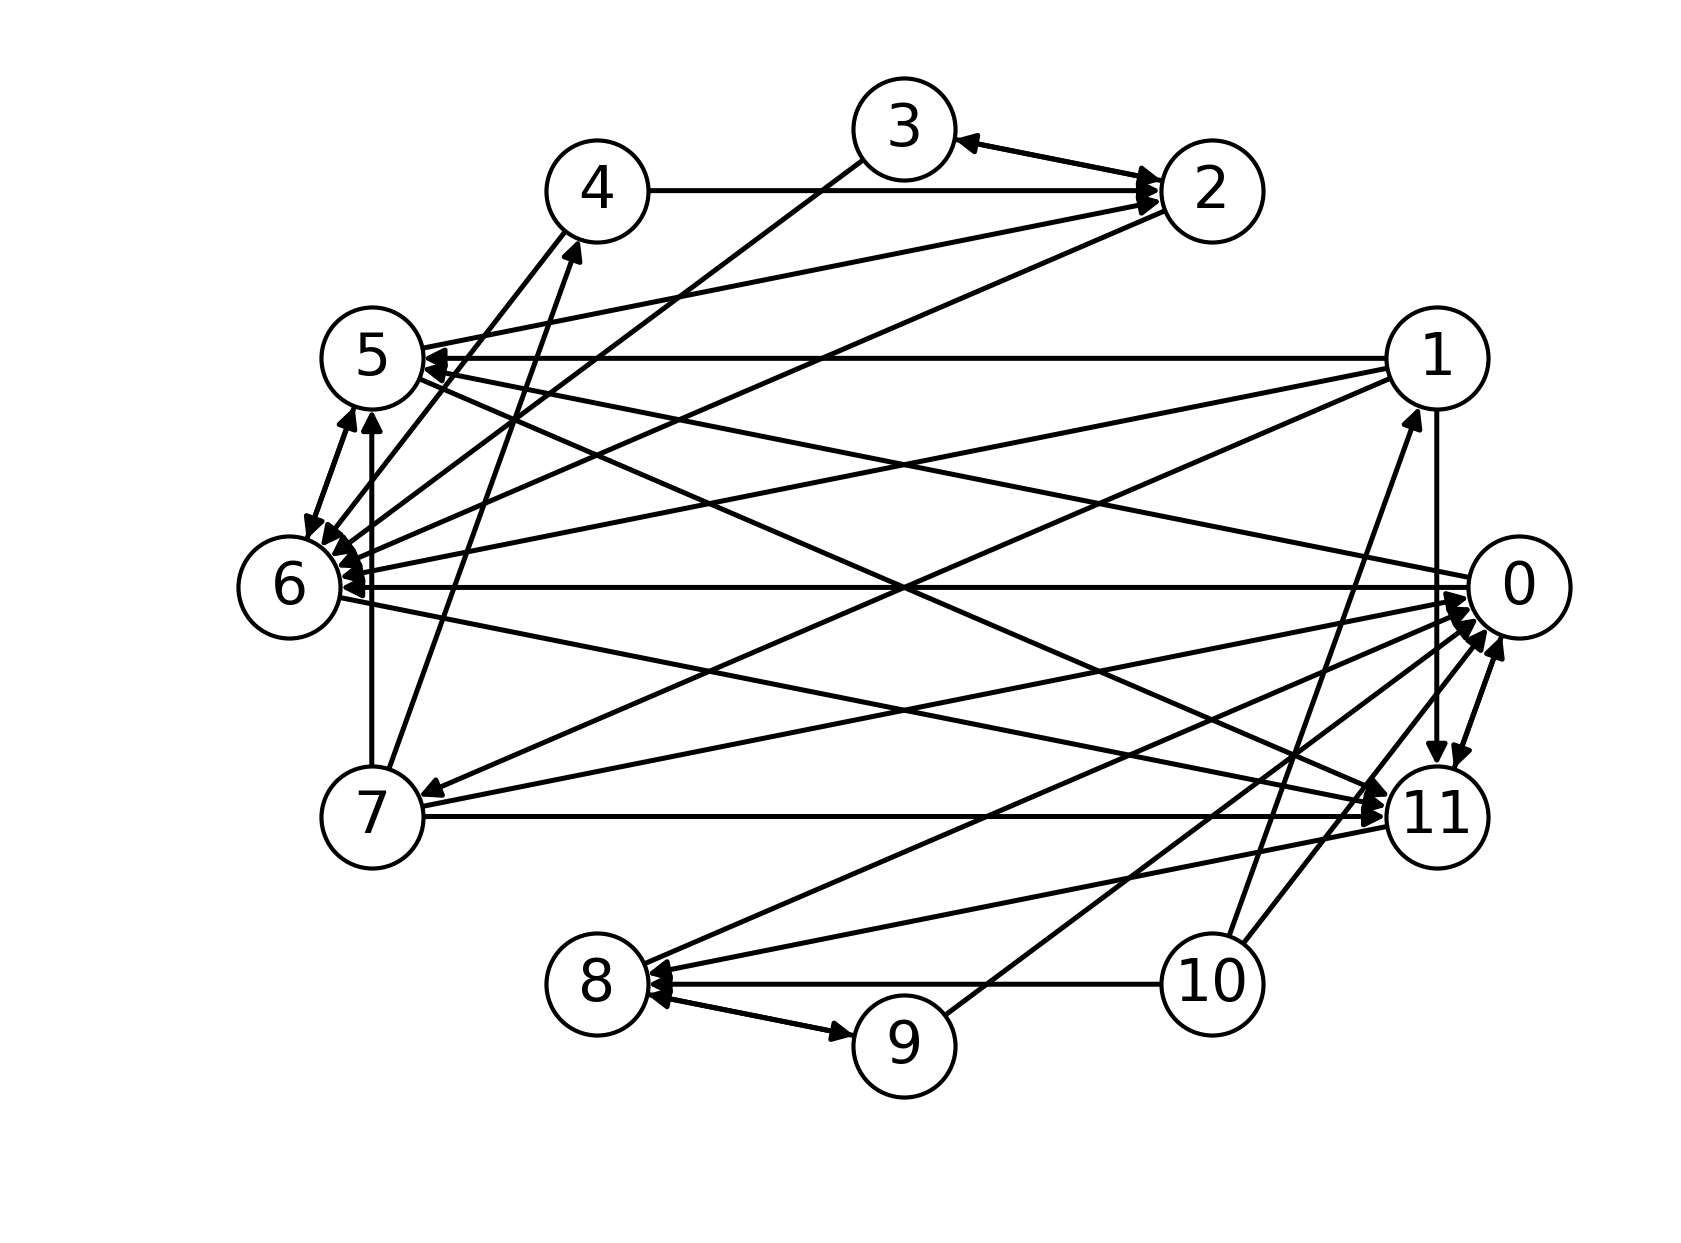
\includegraphics[width=\linewidth]{figures/simple_bit_safe_graph.png}
\end{subfigure}
\caption{A polygon after Algorithm \ref{algo:insert} and the corresponding graph
$BVG_{safe}$. }
\label{fig:simple_bit}
\end{figure}


%\textbf{Making Concise Strategies:}
%In general, deciding whether a given path may be
%executed with $k$ constant fixed bounce rule controllers is the interval
%hitting-set problem, which is NP-hard, though in practice we are mostly
%interested in small $k$. Perhaps some geometric heuristics can be found to solve
%the problem more efficiently in certain cases.


\subsection{Patrolling}

Note that all cycles in the bounce visibility graph for which the contraction coefficient of
the cycle is less than 1 in magnitude will induce limit cycles. There are
exponentially many possible limit cycles, since a cycle may contain
transitions which are not contraction mappings. We may search this space of cycles to
solve various robotic tasks. We define the \emph{patrolling} task as:

\begin{definition}
Given an environment $P$, a set of possible starting states $S$, and
a sequence of edges of the environment $E = \{e_1, \ldots, e_k\}$,
determine a strategy which causes the robot to visit each edge of the sequence
in order from any point in $S$.
\end{definition}

This task is related to the Aquarium Keeper's Problem in computational
geometry \cite{czyzowicz1991aquarium}. It may be solved by coloring nodes in the
bounce visibility graph by which edge of $P$ they belong to, and then searching
for safe cycles which visit edges in the correct order. If a cycle is
contracting, it will result in a converging stable trajectory. 
We may also define another patrolling task:

\begin{proposition}
Given any polygon $P$, a set of possible starting states $S$, 
there exists a strategy $\pi$ such that the robot's trajectory 
converges to a stable limit cycle reachable from all points in $S$.
\end{proposition}

\begin{proof}
Proposition \ref{prop:cycle}
states that a limit cycle is reachable under some constant fixed-angle bounce 
rule from all points in $\partial P$.
\end{proof}

\textbf{Leveraging Cycles to Reduce Uncertainty:}
Say no safe path exists between two subsets of $\partial P$. We may
use limit cycles to reduce the uncertainty in the robot's position enough to
create a safe transition. By Proposition \ref{prop:cycle}, limit cycles are reachable from any point $s
\in \partial P$ under a constant fixed-angle controller (and we know the range
of angles from which this constant controller may be drawn). Say the contraction 
coefficient of a given limit cycle is $C$, and the length of edge $e_i$ is
$\ell_i$. After $k$ iterations of the cycle,
the distance between the robot's position and the fixed point of the cycle's transition
function is less than $C^k \ell_i$. Thus,
we may reduce the uncertainty in the robot's position to less than $\epsilon$
after $\lceil \log(\epsilon/\ell_i)/\log(C) \rceil$ iterations of the 
cycle. If instead of a deterministic fixed-angle controller, we have a
nondeterministic controller with a range of output angles, we need to
compute the resulting range of $C$ coefficients and interval of possible fixed
points, and choose $k$ to be high enough to shrink the robot's location
uncertainty enough to create new safe actions. The best way to choose such
cycles to maximize allowable uncertainty, or minimize $k$, is still an open
question.

%
%Algorithm: finding limit cycles is done by finding cycles in graph with
%contraction coefficient less than 1

%\begin{definition}
%A sequence of transitions $f_1 \circ \ldots \circ f_k$ is \textbf{strongly
%contracting} if $\forall i \in \{1, \ldots, k\}, f_i$ is a contraction mapping.
%\end{definition}
%
%\begin{corollary}
%Every polygon will produce a bounce visibility graph containing at least two
%strongly contracting cycles, for $\theta \in [0, \phi_{min}/2]$ and $\theta \in
%[\pi - \phi_{min}/2, \pi]$.
%\end{corollary}
%
%\begin{proof}
%
%Let the robot have a constant fixed angle bounce strategy, so it always leaves
%the boundary at angle $\theta \in [0,\phi_{min}/2]$ counterclockwise from the
%boundary.
%
%At each transition, the robot will either strike the next adjacent edge in
%$P$, or a reflex vertex will cause the robot to strike some other edge in the
%polygon. Either way, the transition is guaranteed to be a contraction mapping by
%the definition of $\phi_{min}$ and Lemma \ref{lemma:angrange}.
%
%Eventually, this strategy will produce a strongly contracting cycle. Each
%transition moves the robot from one edge to another, so at some point, the
%robot's trajectory must return to an edge it has previously visited. The series
%of transitions in this trajectory corresponds exactly to a strongly contracting
%cycle in the bounce visibility graph.
%\qed
%
%\end{proof}
%
%Note that the previous proof does not guarantee a limit cycle in every polygon.
%It is possible to construct polygons such that the locations of the collision
%points in the stable limit cycle do not all fall within the edges forming the
%strongly contracting cycle. However, the only examples of such that we have been
%able to construct are in general position and are unlikely to occur in practical
%applications.
%
%Note that limit cycles can contain non-contracting bounces, so the number of
%possible limit cycles is exponential in $n$.

\section{Open Questions and Future Work}

We have presented a visibility-based approach to reasoning about 
paths and strategies for a class of mobile robots. We are moving toward
understanding nondeterministic control of such robots; however, many open
questions remain!

\textbf{Comparing bounce rules.} Our approach can be used to compare different families of
bounce strategies in a given polygon, by comparing the reachability of the
transition systems induced by each strategy family. This would require 
either reducing the full bounce visibility graph given constraints on
possible bounces, or constructing a more appropriate transition
system. It is not clear the best way to analyze relative bounce rules, in which the
outgoing angle of a robot after a collision is a function of the incoming angle.
One method would be to choose a subset of configuration space to be the initial
conditions of such a robot, and then propagate this set forward.

\textbf{Optimal Strategies.} Say we wish to
find the strategy taking the robot from region $S$ to region $G$ with the
maximum amount of allowed uncertainty in the bounce rules (the sum of the
interval sizes of each action set along the path). This problem can be framed as
an optimization problem over the space of all transition function compositions.

\textbf{Localization.} A localization strategy is a nondeterministic strategy that 
produces paths which reduce uncertainty in the robot's position to below some
desired threshold, from arbitrarily large starting sets. The use of limit cycles
to produce localizing strategies has been explored in \cite{alam2018space}, and
it would be interesting to take a similar approach with our environment
discretization.

\textbf{Ergodic Trajectories.} 
We are very interested in using the dynamical properties of this robot model to
create controllers that produce ergodic motion, in which the time-averaged
behavior of the system approaches the space-averaged behavior, causing the robot
to not spend ``too much'' time in any given part of the state space. Measures
of ergodicity have recently been used in exploration tasks
\cite{miller2016ergodic}. Chaotic dynamical systems have also been used directly
as controllers for mobile robots \cite{nakamura2001chaotic}.

%\textbf{Obstacles. } There is no obvious reason that Algorithm \ref{algo:insert} and the 
%bounce visibility graph cannot be extended to polygonal regions with obstacles.

\subsubsection{Acknowledgement} This work was supported by NSF grants 1035345 and 1328018, and CONACyT
post-doctoral fellowship 277028.

%When Algorithm \ref{algo:insert} is run, it produces a partition of $P$, where
%two points in the same segment induce visibility polgons which are
%
%One may ask if iterating Algorithm \ref{algo:insert} will produce a 
%
%While they may belong to multiple partitions, the number
%of partitions can be computed by iterating Algorithm \ref{algo:insert}. In some
%polygons, Algorithm \ref{algo:insert} terminates after one iteration; in others,
%it appears to asymptotically approach a partition but never converge. While
%theoretically interesting, the partitions under iteration quickly become too
%small to be practical in our application areas.



%\subsection{Optimal Backprojections for Navigation}
%
%To create a complete navigation algorithm, we 
%
%We have three degrees of freedom when computing action preimages - the angle
%interval and the size/location of the subinterval.
%
%There are two natural quantities we may wish to maximize for such a transition -
%the size of the subinterval, or the size of the angle interval.
%The maximum angle interval will always be a point. Imagine an interval on $e_i$
%which allowed for a maximal angle range $[\theta_{min}, \theta_{max}]$ that
%guaranteed a transition from any point in the interval to $e_j$. By
%shrinking this interval to a point, we must increase the size of the angle
%interval, creating a contradiction. The maximum size subinterval will always correspond to a singleton angle range,
%$\theta$, such that $l_{sub}$ and $r_{sub}$ are parallel. The location of this
%interval will depend on the local geometry.
%
%Case 1: start set is entirely contained within equivalence class
%
%Case 2: start set is split across equivalence classes (make strategies for
%subsets of start set and intersect - what kinds of strategy intersections make
%sense?)


%\subsubsection{Incorporating other Sensor Models}
%
%\section{Examples}
%
%\subsection{office space w/ long hallway}
%\subsection{``almost symmetric" environment}
%\subsection{worst case complexity}
%

\bibliographystyle{spmpsci}
\bibliography{refs}

\newpage
\section{Appendix}

\begin{appendix}


\section{Proof of Proposition \ref{prop:complexity}}


\textbf{Proposition 1.} {\em The bounce visibility graph for a simple polygon with $n$ vertices has 
$O(n^2)$ vertices and $O(n^4)$ edges.}

\begin{proof}

Consider a polygon $P$ with $n$ vertices, $r$ of which are reflex vertices. To
construct the bounce visibility graph, we insert the vertices of the partial
local sequence for each vertex in $P$. For a convex vertex, its partial local sequence 
will not add any new vertices to $P$. However, a reflex vertex can add $O(n)$ new vertices. 

Up to half of the vertices in the polygon can be reflex, so the complexity of
$r$ is $O(n)$. Therefore, the number of vertices in $P'$, returned by Algorithm
\ref{algo:insert} is $O(n^2)$. Each vertex indexes an edge in $P'$, and
thus a node in the edge visibility graph of $P'$. At most, a given vertex in $P'$ may see all other vertices, so in the worst
case, the bounce visibility graph will have $O(n^4)$ edges. See Figure
\ref{fig:alg1} for an example of such a polygon. \qed

\end{proof}

\subsection{Worst Case Example for Algorithm \ref{algo:insert}}

We might hope that if $r$ is large, then not all of the reflex vertices will
produce a large number of new vertices, and we may bound the size of the edge
set in the visibility graph. Unfortunately, the number of reflex
vertices, the new vertices produced in their partial local sequence, and the new
vertices' visibility can be large at the same time. We will present a family of
input polygons with bounce visibility graph edge-set size of $O(n^4)$.

Let $n = 4t+2$, in which $t$ is a positive integer. We design a polygon with
$r = 2t$ reflex vertices. The polygon is symmetric with respect to its medium
horizontal line. In the top half, the reflex vertices are uniformly located on a
circle and thus they are visible to each other; the convex vertices are chosen
so that they are outside the circle and the line through an edge will not
intersect other edges. Each reflex vertex will have at least $t-1$ new
vertices in its partial local sequence. There will be $2t(t-1)+n$
vertices in the polygon after we insert all new vertices in the partial local
sequence for all reflex vertices. Each of them can see at least $t(t-1)+n/2$
other vertices. Thus the number of edges in the transition graph for the
polygon with inserted vertices is
$O ((2t(t-1)+n)(t(t-1)+n/2)) = O(t^4) = O(n^4)$.
Fig \ref{fig:alg1} shows the polygon for $t = 4$ with all the
vertices in the partial local sequences. % show the diagram to edge

\section{Proof of Proposition \ref{prop:saferange}}

\textbf{Proposition 2.} {\em
Given two entirely visible line segments $e_i = (v_i, v_{i+1})$ and $e_j =
(v_j, v_{j+1})$, if a safe action
exists from $e_i$ to $e_j$, the maximum range of safe actions is $\bm{\tilde{\theta} = [\theta_r, \theta_l]}$ such
that $\theta_r = \pi - \angle v_j v_{i+1} v_i$ and $\theta_l = \angle v_{j+1}
v_i v_{i+1}$.}

\begin{proof}

Let edge $e_i = (v_i, v_{i+1})$ be aligned with the positive $x$ axis with the clockwise
endpoint at the origin, without loss of generality. 
Due to the edges being
entirely visible, $e_j = (v_j, v_{j+1})$ must be in the top half of the plane, above
$e_i$.

Take the quadrilateral formed by the convex hull of the edge endpoints.
Let the edges between $e_i$ and $e_j$ be $e_l = (v_i, v_{j+1})$ and the right-hand edge 
$e_r = (v_{i+1}, v_j)$. Let $\theta_{l}$ be
the angle between $e_l$ and the positive $x$ axis ($0 < \theta_l < \pi$); similarly
for $e_r$ and $\theta_r$. See Figure \ref{fig:bounce_range} for an illustration of
the setup. 

\begin{figure}
    \centering
    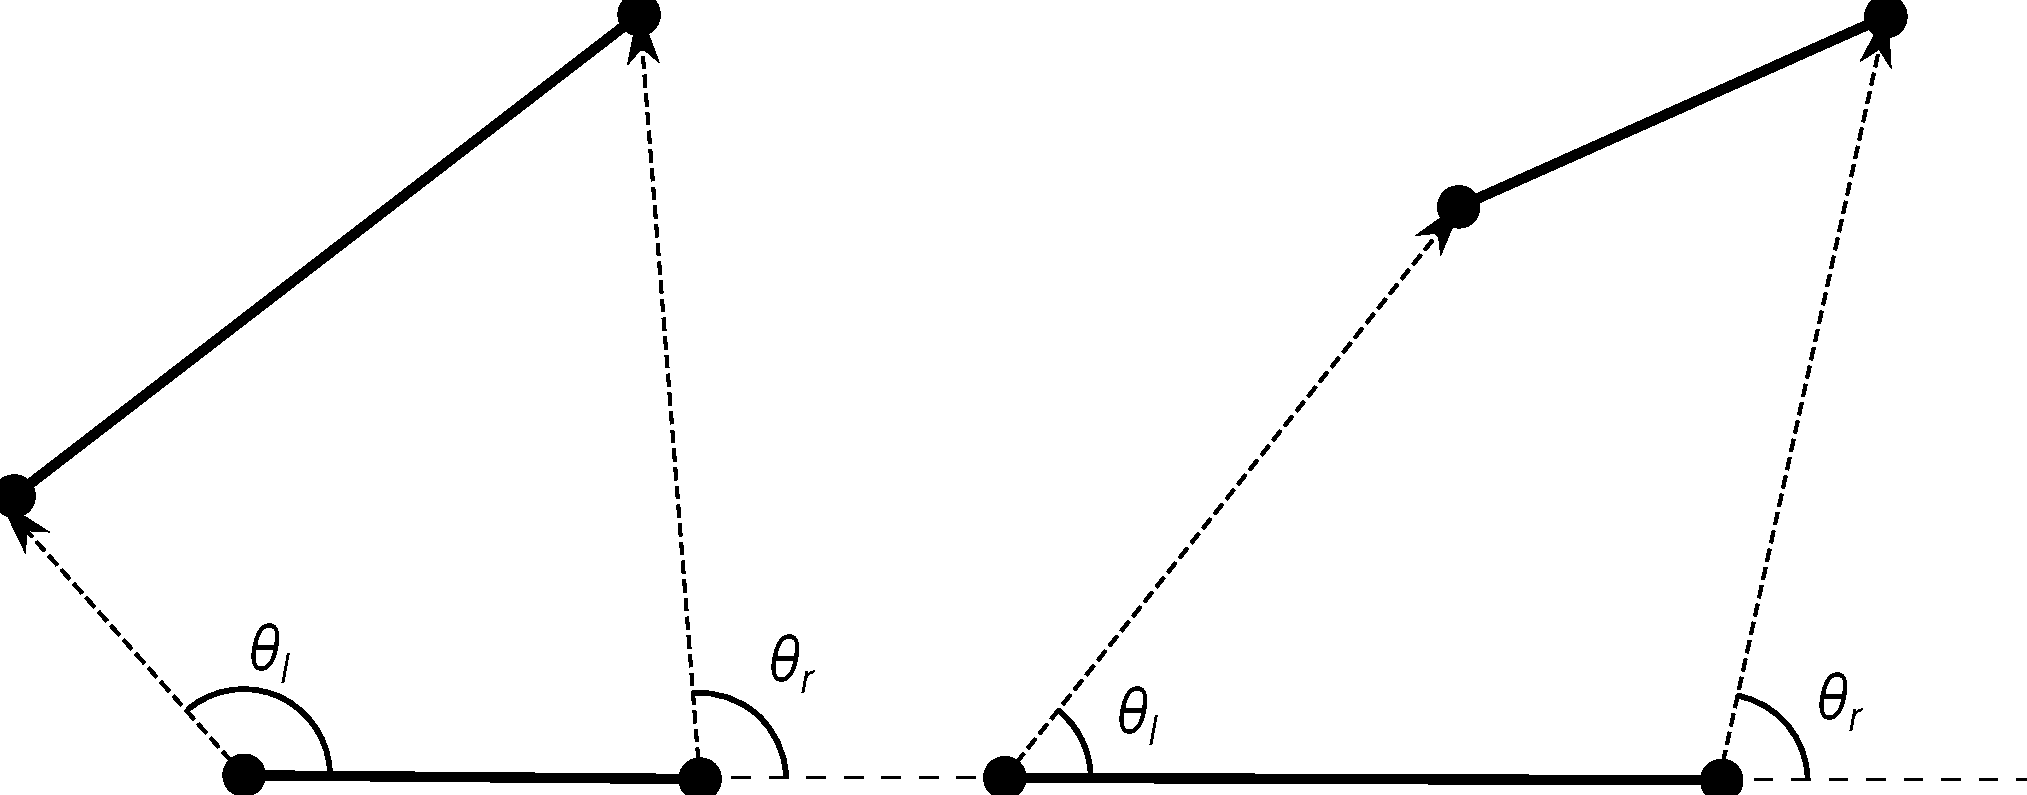
\includegraphics[width=0.7\linewidth]{figures/bouncerange_min.pdf}
    \caption{Angle range such that a transition exists for all points on
originating edge (left: such a range exists, right: such a range does not
exist)}
\label{fig:bounce_range}
\end{figure}


There are three cases to consider: if $e_l$ and $e_r$ are extended to infinity,
they cross either above or below edge $e_i$, or they are parallel.

\emph{Case 1:} $e_l$ and $e_r$ meet below edge $e_i$. In this case,
$\theta_l > \theta_r$ and if a ray is cast from any point on $e_i$ at angle
$\theta \in [\theta_r, \theta_l]$, the ray is guaranteed to intersect $e_j$ in its
interior.

\emph{Case 2:} $e_l$ and $e_r$ meet above edge $e_i$. In this case, $\theta_l <
\theta_r$, and there is no angle
$\theta$ such that a ray shot from \emph{any} point on $e_i$ will intersect
$e_j$.
To see this, imagine sliding a ray at angle $\theta_l$ across the quadrilateral
- at some point before reaching $v_{i+1}$, the ray must stop intersecting $e_j$,
else we would have $\theta_l > \theta_r$.

\emph{Case 3:} $e_l$ and $e_r$ are parallel. This implies that $\theta_{l} =
\theta_{r}$, which is the only angle for which a transition from any
point on $e_i$ is guaranteed to intersect $e_j$, and $\tilde{\theta}$ is a
singleton set.

Thus, for each case, we can either compute the maximum angle range or determine
that no such angle range exists.
\qed

\end{proof}

\section{Proof of Lemma 1}

\textbf{Lemma 1.} {\em
If two segments are entirely visible to each other, there will be at least one safe
action between them.}

\begin{proof}
From the proof of Proposition \ref{prop:saferange}, we can see that if case one
holds in one direction, case two will hold in the other direction, so a safe
action must exist from one edge to the other in one direction. If case three
holds, there is a safe action both directions but $\tilde{\theta}$ is a
singleton set.
\end{proof}
\section{Proof of Lemma \ref{lemma:angrange}}

\textbf{Lemma 2.} {\em
If the transition from segment $e_i$ to segment $e_j$ is a left transition, then the
transition function $f(x, \theta)$ between segments $e_i$ and $e_j$ is a contraction
mapping if and only if $\theta > \frac{\pi}{2}+\frac{\phi_{i, j}}{2}$;
otherwise, the transition function $f(x, \theta)$ is a contraction mapping if
and only if $\theta < \frac{\pi}{2}-\frac{\phi_{i, j}}{2}$.}

\begin{proof}

\begin{figure}
    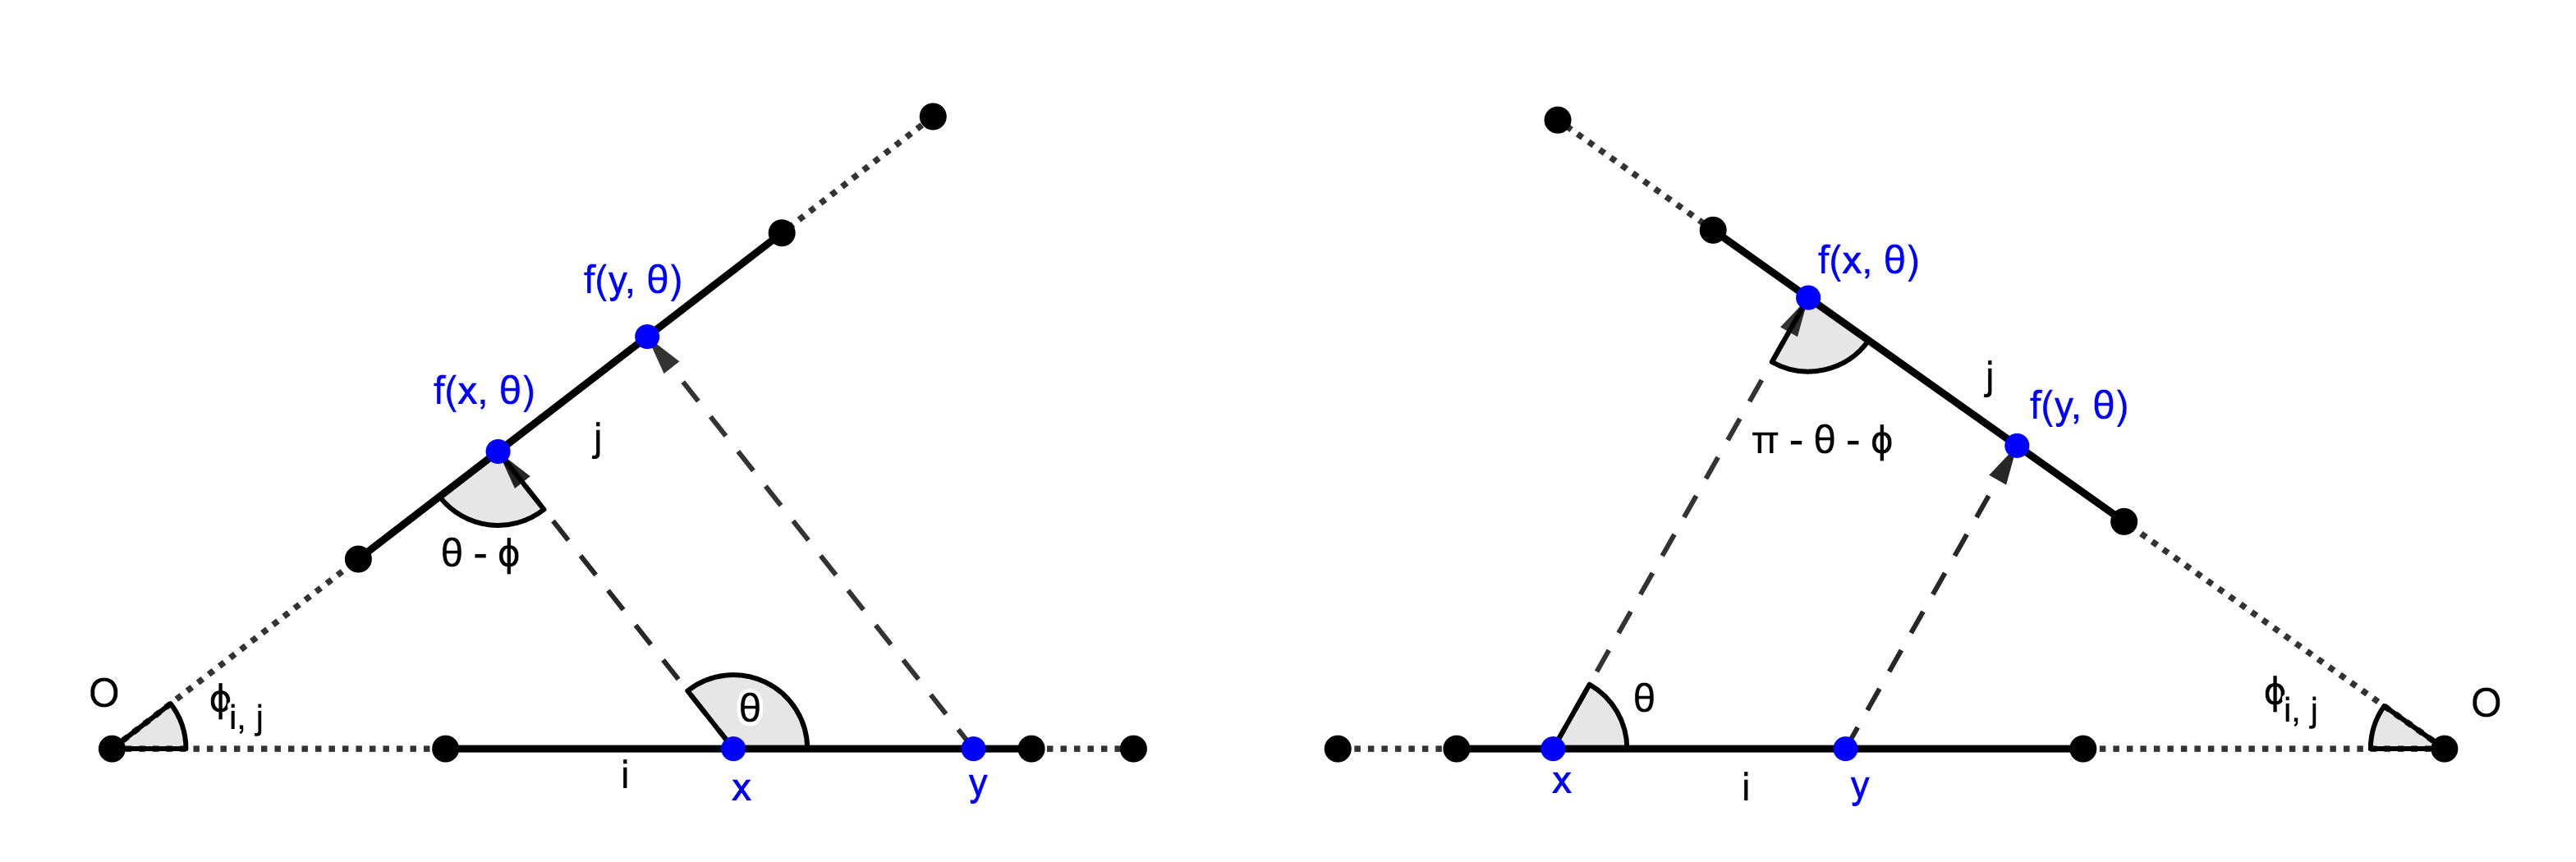
\includegraphics[width=1\linewidth]{figures/contraction_map_cond.png}
    \centering
    \caption{The two cases for computing contraction mapping conditions. \label{fig:cont_map}}
    \centering
\end{figure}

We consider the two cases of transition separately:
\begin{enumerate}
    \item For the transition shown in the left hand side of Figure~\ref{fig:cont_map}, 
          $\overline{xf(x, \theta)} \parallel \overline{yf(y, \theta)} \Rightarrow \frac{|f(x, \theta)-f(y, \theta)|}{|x-y|} = \frac{|f(x, \theta)|}{|x|} = \frac{\sin(\pi - \theta)}{\sin(\theta - \phi_{i, j})} = \frac{\sin(\theta)}{\sin(\theta-\phi_{i, j})}.$ The transition will be contraction if and only if $\frac{|f(x, \theta)-f(y, \theta)|}{|x-y|} < 1 \iff \sin(\theta)<\sin(\theta-\phi_{i, j})$. If $\theta < \frac{\pi}{2}$, then $\sin(\theta) > \sin(\theta-\phi_{i, j})$. Thus we need $\theta>\frac{\pi}{2}$. If $\theta-\phi_{i, j} > \frac{\pi}{2}$, then $\sin(\theta) < \sin(\theta-\phi_{i, j})$ and we are done; otherwise we need $\pi - \theta < \theta-\phi_{i, j} \Rightarrow \theta - \frac{\phi_{i, j}}{2} > \frac{\pi}{2}$. Combining all conditions, we have the transition will be contraction if and only if $\theta >\frac{\pi}{2} + \frac{\phi_{i, j}}{2}$.
    \item Similarly, for a right transiton shown in the right diagram of figure~\ref{fig:cont_map}, $\overline{xf(x, \theta)} \parallel \overline{yf(y, \theta)} \Rightarrow \frac{|f(x, \theta)-f(y, \theta)|}{|x-y|} = \frac{|f(x, \theta)|}{|x|} = \frac{\sin(\pi - \theta)}{\sin(\pi -\theta-\phi_{i, j})} = \frac{\sin(\theta)}{\sin(\theta + \phi_{i, j})}.$ The transition will be contraction if and only if $\frac{|f(x, \theta)-f(y, \theta)|}{|x-y|} < 1 \iff \sin(\theta)<\sin(\theta+\phi_{i, j})$. If $\theta  > \frac{\pi}{2}$, then $\sin(\theta) > \sin(\theta + \phi_{i, j})$. Thus we need $\theta<\frac{\pi}{2}$. If $\theta+\phi_{i, j} < \frac{\pi}{2}$, then $\sin(\theta) < \sin(\theta+\phi_{i, j})$ and we are done; otherwise we need $\theta < \pi-\theta-\phi_{i, j} \Rightarrow \theta < \frac{\pi}{2} - \frac{\phi_{i, j}}{2}$. Combining all conditions, we have the transition will be contraction if and only if $\theta <\frac{\pi}{2} - \frac{\phi_{i, j}}{2}$.
\end{enumerate}
\qed

\newpage

\section{Supplementary Figure for Theorem \ref{thm:convex}}

\begin{figure}
    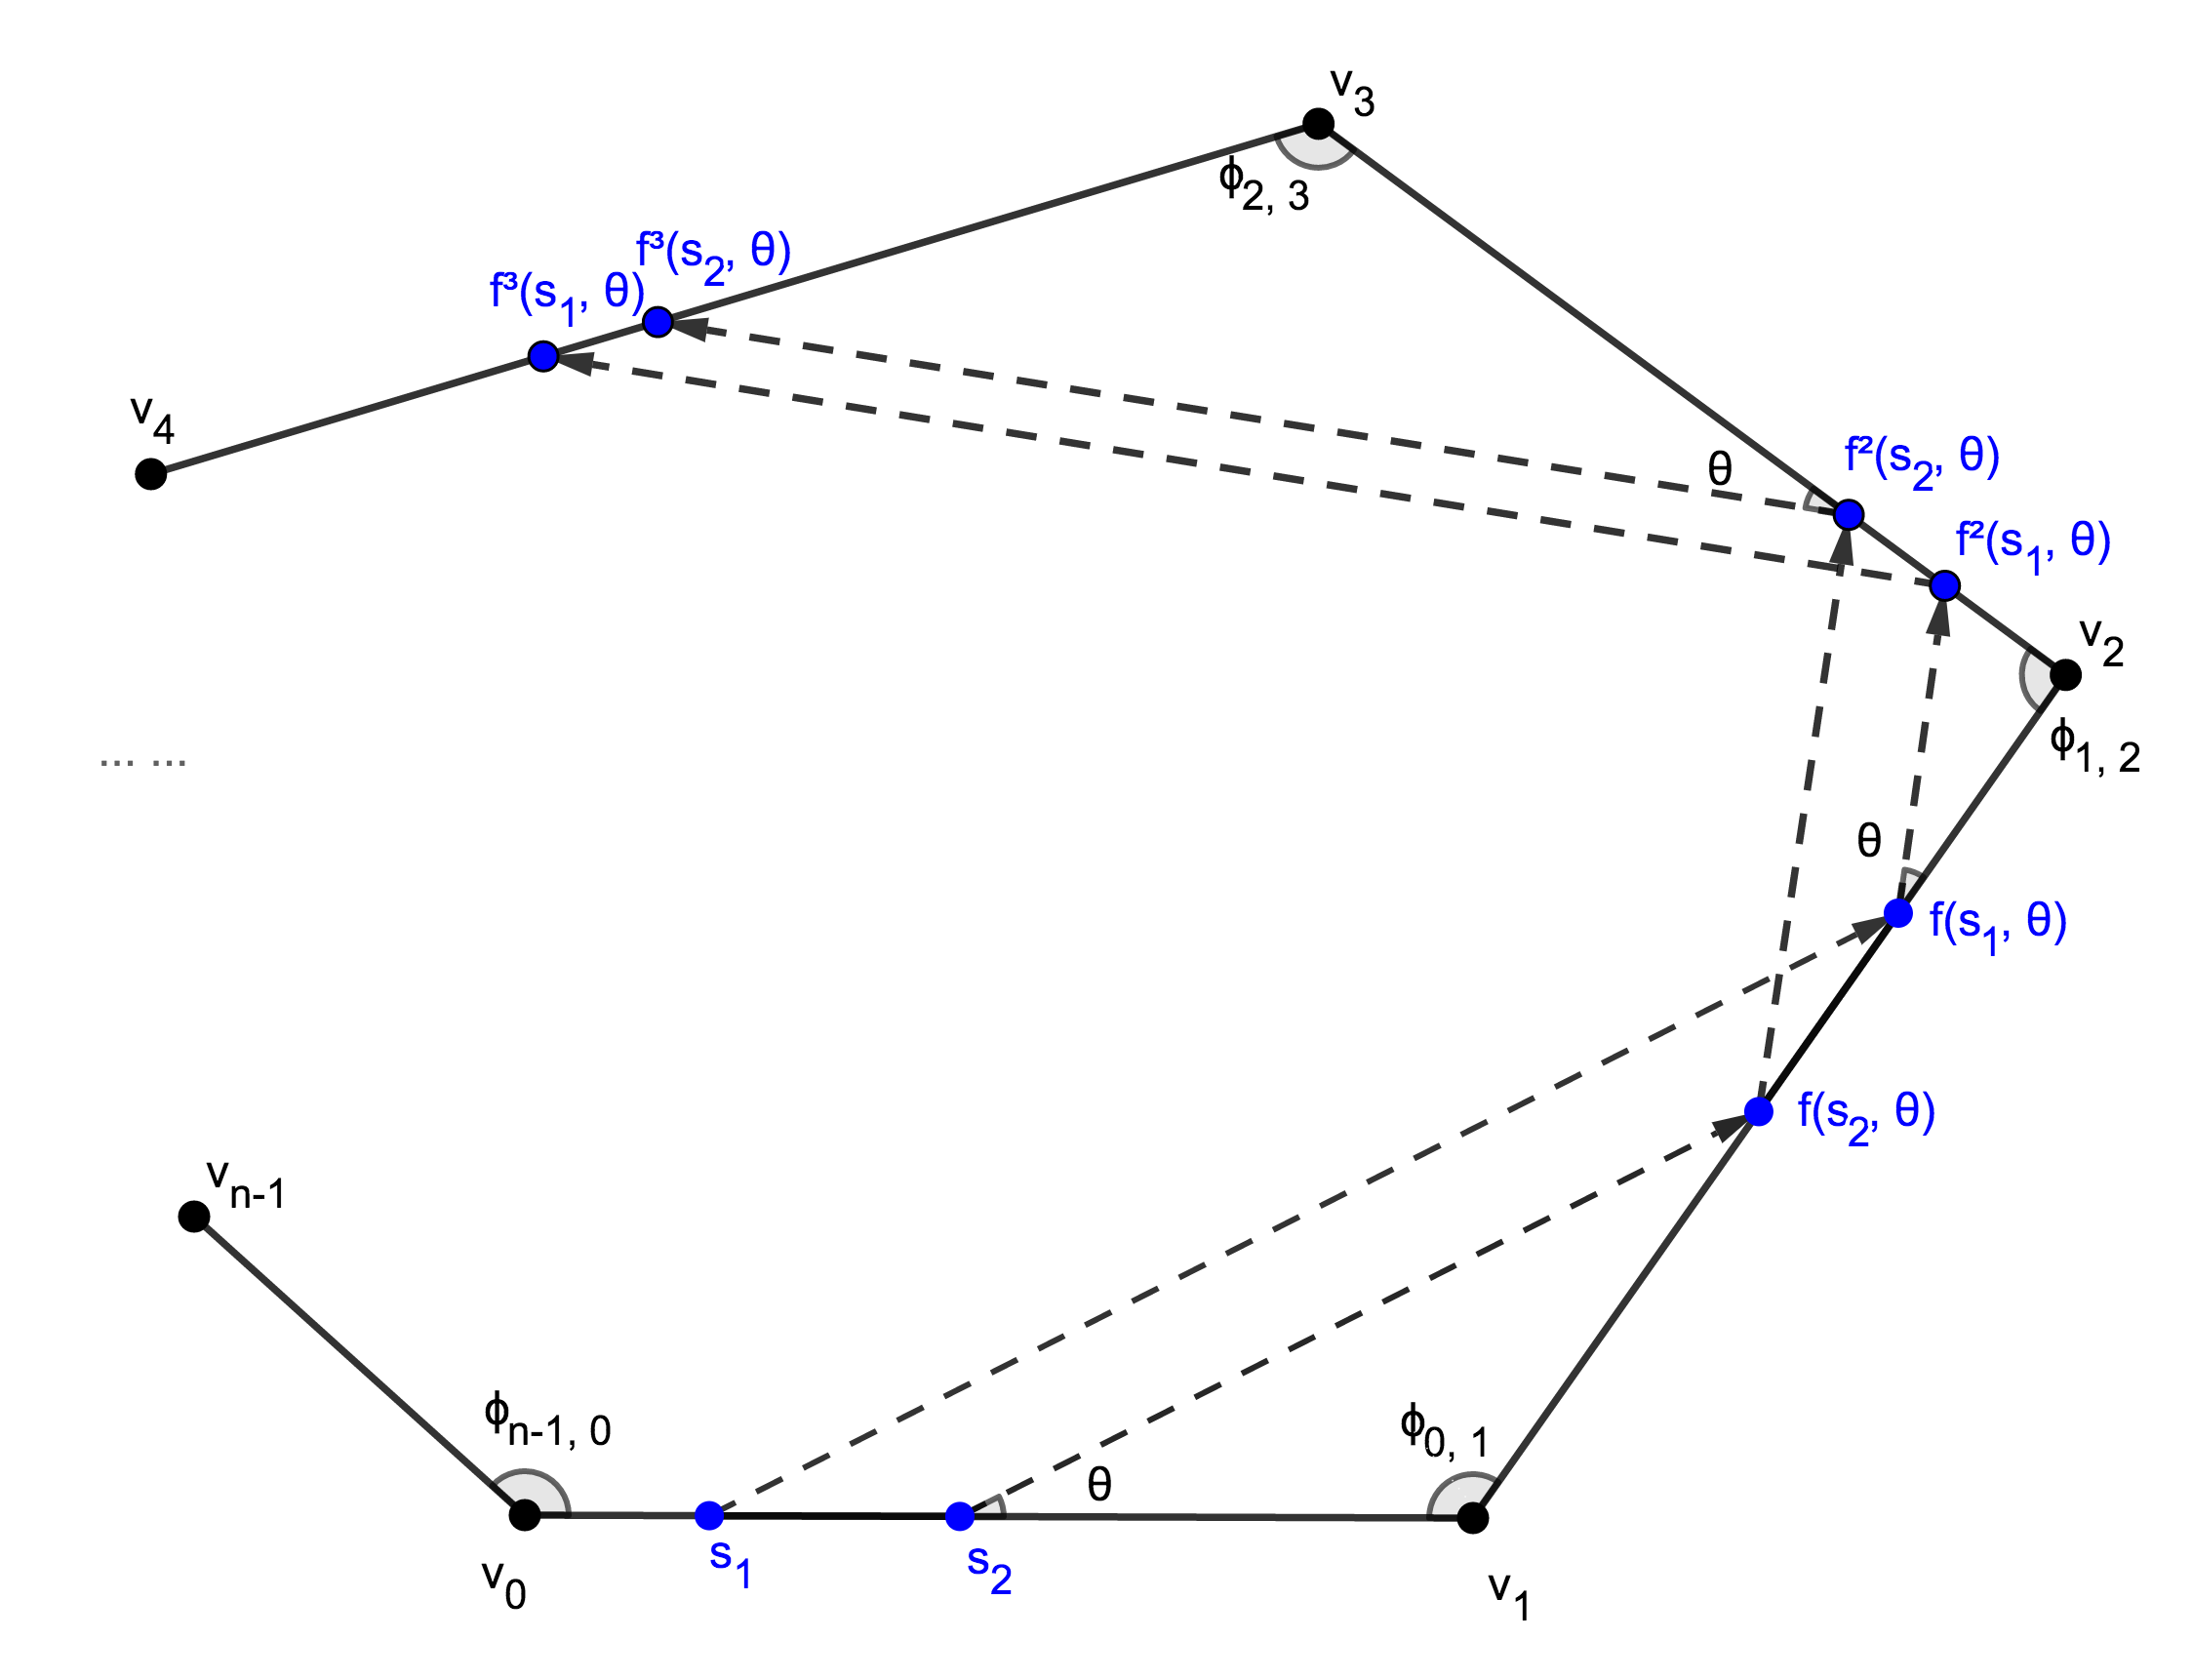
\includegraphics[width=0.6\linewidth]{figures/convex_cycle.png}
    \centering
    \caption{The notation setup for the proof of contracting cycle in a convex polygon.\label{fig:conv_cycle}}
    \centering
\end{figure}

%\begin{figure}
%    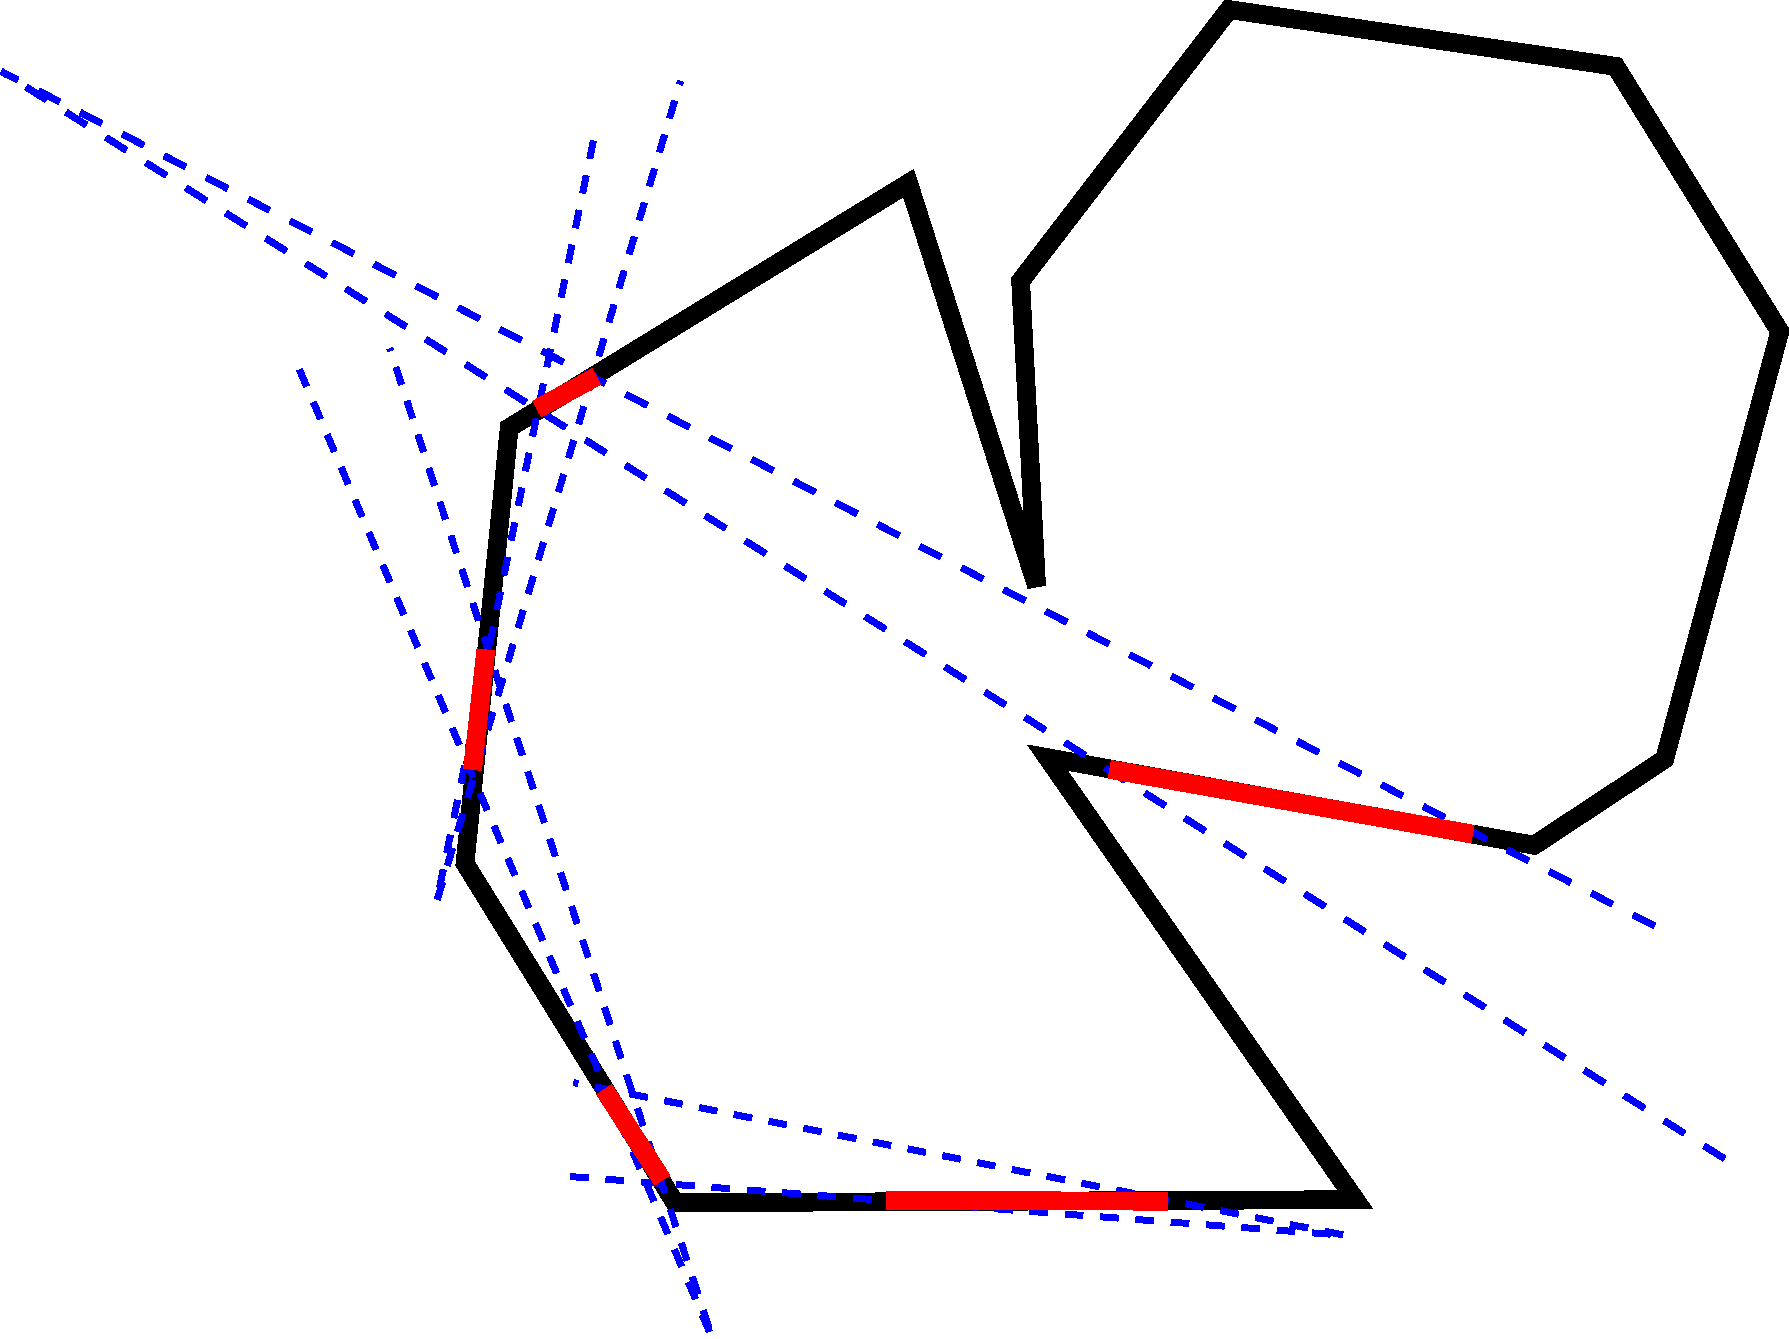
\includegraphics[width=0.6\linewidth]{figures/bounce_preimages.pdf}
%    \centering
%    \caption{An example of how contraction properties can be used to control
%robot state uncertainty enough to navigate the robot through a narrow doorway,
%even with a lower bound on angle error.}
%\label{fig:preimage_example}
%\end{figure}


\end{proof}

\end{appendix}

\end{document}
